% !TEX TS-program = lualatex
% !TEX encoding = UTF-8 Unicode		

\documentclass[12pt, letterpaper]{article}

%%BIBLIOGRAPHY- This uses biber/biblatex to generate bibliographies according to the 
%%Unified Style Sheet for Linguistics
\usepackage[main=american, german]{babel}% Recommended
\usepackage{csquotes}% Recommended
\usepackage[backend=biber,
		style=unified,
		maxcitenames=3,
		maxbibnames=99,
		natbib,
		url=false]{biblatex}
\addbibresource{Library.bib}
\setcounter{biburlnumpenalty}{100}  % allow URL breaks at numbers
%\setcounter{biburlucpenalty}{100}   % allow URL breaks at uppercase letters
%\setcounter{biburllcpenalty}{100}   % allow URL breaks at lowercase letters

%%TYPOLOGY
\usepackage[svgnames]{xcolor} % Specify colors by their 'svgnames', for a full list of all colors available see here: http://www.latextemplates.com/svgnames-colors
%\usepackage[compact]{titlesec}
%\titleformat{\section}[runin]{\normalfont\bfseries}{\thesection.}{.5em}{}[.]
%\titleformat{\subsection}[runin]{\normalfont\scshape}{\thesubsection}{.5em}{}[.]
\usepackage[hmargin=1in,vmargin=1in]{geometry}  %Margins          
\usepackage{graphicx}	%Inserting graphics, pictures, images 		
\usepackage{stackengine} %Package to allow text above or below other text, Also helpful for HG weights 
\usepackage{fontspec} %Selection of fonts must be ran in XeLaTeX or LuaLaTeX
\usepackage{amssymb} %Math symbols
\usepackage{amsmath} % Mathematical enhancements for LaTeX
\usepackage{setspace} %Linespacing
\usepackage{multicol} %Multicolumn text
\usepackage{enumitem} %Allows for continuous numbering of lists over examples, etc.
\usepackage{multirow} %Useful for combining cells in tablesbrew 
\usepackage{booktabs}
\usepackage{hanging}
\usepackage{fancyhdr} %Allows for the 
\pagestyle{fancy}
\fancyhead[L]{\textit{QP draft}} 
\fancyhead[R]{\textit{\today}} 
\fancyfoot[L,R]{} 
\fancyfoot[C]{\thepage} 
\renewcommand{\headrulewidth}{0.4pt}
\setlength{\headheight}{14.5pt} % ...at least 14.49998pt
% \usepackage{fourier} % This allows for the use of certain wingdings like bombs, frowns, etc.
% \usepackage{fourier-orns} %More useful symbols like bombs and jolly-roger, mostly for OT
\usepackage[colorlinks,allcolors={black},urlcolor={blue}]{hyperref} %allows for hyperlinks and pdf bookmarks
% \usepackage{url} %allows for urls
% \def\UrlBreaks{\do\/\do-} %allows for urls to be broken up
\usepackage[normalem]{ulem} %strike out text. Handy for syntax
\usepackage{tcolorbox}
\usepackage{datetime2}
\usepackage{caption}
\usepackage{subcaption}

%%FONTS
\setmainfont{Libertinus Serif}
\setsansfont{Libertinus Sans}
\setmonofont[Scale=MatchLowercase]{Libertinus Mono}

%%PACKAGES FOR LINGUISTICS
%\usepackage{OTtablx} %Generating tableaux with using TIPA
\usepackage[noipa]{OTtablx} % Use this one generating tableaux without using TIPA
%\usepackage[notipa]{ot-tableau} % Another tableau drawing packing use for posters.
% \usepackage{linguex} % Linguistic examples
% \usepackage{langsci-linguex} % Linguistic examples
\usepackage{langsci-gb4e} % Language Science Press' modification of gb4e
% \usepackage{langsci-avm} % Language Science Press' AVM package
\usepackage{tikz} % Drawing Hasse diagrams
% \usepackage{pst-asr} % Drawing autosegmental features
\usepackage{pstricks} % required for pst-asr, OTtablx, pst-jtree.
% \usepackage{pst-jtree} 	% Syntax tree draawing software
% \usepackage{tikz-qtree}	% Another syntax tree drawing software. Uses bracket notation.
\usepackage[linguistics]{forest}	% Another syntax tree drawing software. Uses bracket notation.
% \usepackage{ling-macros} % Various linguistic macros. Does not work with linguex.
% \usepackage{covington} % Another linguistic examples package.
\usepackage{leipzig} %	Offers support for Leipzig Glossing Rules

%%LEIPZIG GLOSSING FOR ZAPOTEC
\newleipzig{el}{el}{elder}	% Elder pronouns
\newleipzig{hu}{hu}{human}	% Human pronouns
\newleipzig{an}{an}{animate}	% Animate pronouns
\newleipzig{in}{in}{inanimate}	% Inanimate pronouns
\newleipzig{pot}{pot}{potential}	% Potential Aspect
\newleipzig{cont}{cont}{continuative}	% Continuative Aspect
% \newleipzig{pot}{pot}{potential}	% Potential Aspect
\newleipzig{stat}{stat}{stative}	% Potential Aspect
\newleipzig{and}{and}{andative}	% Andative Aspect
\newleipzig{ven}{ven}{venative}	% Venative Aspect
% \newleipzig{res}{res}{restitutive}	% Restitutive Aspect
\newleipzig{rep}{rep}{repetitive}	% Repetitive Aspect

%%TITLE INFORMATION
\title{QP2}
\author{Mykel Loren Brinkerhoff}
\date{\today}

%%MACROS
\newcommand{\sub}[1]{\textsubscript{#1}}
\newcommand{\supr}[1]{\textsuperscript{#1}}
\providecommand{\lsptoprule}{\midrule\toprule}
\providecommand{\lspbottomrule}{\bottomrule\midrule}
\newcommand{\fittable}[1]{\resizebox{\textwidth}{!}{#1}}

\makeatletter
\renewcommand{\paragraph}{%
  \@startsection{paragraph}{4}%
  {\z@}{0ex \@plus 1ex \@minus .2ex}{-1em}%
  {\normalfont\normalsize\bfseries}%
}
\makeatother
\parindent=10pt


\begin{document}
	
%%If using linguex, need the following commands to get correct LSA style spacing
%% these have to be after  \begin{document}
	% \setlength{\Extopsep}{6pt}
	% \setlength{\Exlabelsep}{9pt}		%effect of 0.4in indent from left text edge
%%
	
%% Line spacing setting. Comment out the line spacing you do not need. Comment out all if you want single spacing.
%	\doublespacing
	\onehalfspacing
	
\begin{center}
	{\Large \textbf{Investigating the timing of tone and phonation in Santiago Laxopa Zapotec}}\footnote{I am grateful to Fe Silva-Robles and  Raúl Díaz Robles for sharing their time and language expertise. I am also grateful to Grant McGuire,  Jaye Padgett, Rachel Walker, Maziar Toosarvandani, Ben Eischens, Kim Tan, and Zach Horton for their help and discussions during all stages of this project. This project branched off from a collaboration with  Jack Duff and Maya Wax Cavallaro. Various parts of this project were previously shared in joint presentations with Jack Duff and Maya Wax Cavallaro.
	
	This work was supported in part by the National Science Foundation under Grant No. 2019804, the Humanities Institute at UC Santa Cruz, and the Jacobs Research Funds.}
	\vspace{6pt}

	Mykel Loren Brinkerhoff
\end{center}
%\maketitle
%\maketitleinst
\thispagestyle{fancy}

% \tableofcontents


%------------------------------------
\section{Introduction} \label{sec:Introduction}
%------------------------------------

Most of the work on the interaction of tone and phonation has been based on descriptions of Southeast and Far East Asian languages, which lead to strong claims being made about what is possible for the interaction between tone and phonation \citep{masicaDefiningLinguisticArea1976,thurgoodVietnameseTonogenesisRevising2002,yipTone2002,enfieldArealLinguisticsMainland2005,michaudComplexTonesEast2012,brunelleTonePhonationSoutheast2016}. The main claim from many of these authors is that tone and phonation are codependent (i.e., certain tones only appear with certain phonations or certain phonations only appear with certain tones).

An example for this type of co-occurrence between tone and phonation is Mandarin's Tone 3 which is frequently associated with creaky voice \citep{hockettPeipingPhonology1947,}. This claim has also been made in the reverse that certain phonation types are associated with specific tonal patterns. Breathy voice stereotypically appears with high pitch and creaky voice stereotypically appears with low pitch \citep{eslingVoiceQualityLaryngeal2019}.

Research into Mesoamerican languages, however, shows that these claims are too strong or exaggerated \citep{suarezMesoamericanIndianLanguages1983,campbellMesoAmericaLinguisticArea1986,silvermanLaryngealComplexityOtomanguean1997,dicanioPhoneticsPhonologySan2008,espositoVariationContrastivePhonation2010, campbellOtomangueanHistoricalLinguistics2017a,campbellOtomangueanHistoricalLinguistics2017}. 
Most languages of the Oto-Manguean language family exhibits independent tone and phonation. This has lead some researchers to propose that tone and phonation is phased/ordered with respect to each other \citep{silvermanLaryngealComplexityOtomanguean1997,blankenshipTimeCourseBreathiness1997,blankenshipTimingNonmodalPhonation2002}. A summary of this proposal, which I call the Laryngeal Complexity 

This paper presents novel data on the interaction of tone and phonation in Santiago Laxopa Zapotec, an Oto-Manguean language spoken in Santiago Laxopa, Ixtlán, Oaxaca, Mexico. This paper presents a brief description of the tone and phonation systems of the language. The result of the a statistical analysis shows that the tone and phonation is phased with respect to each other. 
% \begin{itemize}
% 	\item This paper adds to this debate by:
% 	\begin{itemize}
% 		\item Providing another description of a language that uses tone and phonation
% 		\item Evaluates the claims of \citet{silvermanLaryngealComplexityOtomanguean1997}
% 	\end{itemize}
% \end{itemize}

%------------------------------------
\section{The Laryngeal Complexity Hypothesis} \label{sec:Silverman}
%------------------------------------

The \textsc{Laryngeal Complexity Hypothesis} (LCH) has it origins in the work from \citet{silvermanLaryngealComplexityOtomanguean1997,blankenshipTimeCourseBreathiness1997,blankenshipTimingNonmodalPhonation2002}. The basic premise of the LCH is that in languages that have both tone and phonation there needs to be an ordering between the two laryngeal gestures for tone and phonation for optimal perceptibility. This premise comes from the understanding that the same mechanism that is responsible for tone is also responsible for the production of phonation: the vocal folds and glottis. The rate that vocal folds vibrate is responsible for changing the fundamental frequency, perceived as pitch, which is grammaticalized as tone in lexical tone languages. The faster the vocal folds vibrate the higher the pitch and the slower the vocal folds vibrate the lower the pitch. 

The vocal folds are also the primary articulator for phonation. \citet{ladefogedPreliminariesLinguisticPhonetics1971,gordonPhonationTypesCrosslinguistic2001} treated phonation as a by-product of how open or closed the glottis is during vocal fold vibration. This is schematized by Figure~\ref{fig:Phonation}. The more open the glottis is the breathier the sound to the point where the sound becomes the sound [h]. The more closed the glottis is the creakier the sound is to the point where the sound becomes [ʔ]. 
\begin{figure}[!ht]
	\centering
	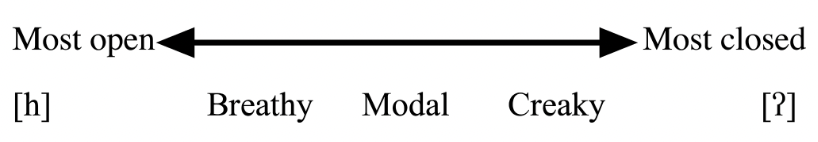
\includegraphics[width=.6\textwidth]{../Phonation.png}
	\caption{Simplified one-deminsional model for phonation. Based on \citet{ladefogedPreliminariesLinguisticPhonetics1971,gordonPhonationTypesCrosslinguistic2001}}.
	\label{fig:Phonation}
\end{figure}
\vspace{-2ex}

The LCH assumes that phonation and tone are both produced at the vocal folds and glottis. Because these same organs are responsible for these two different phenomena there is a mismatch in trying to produce both at the same time. It is assumed by the LCH that because of this issue there needs to be a strict ordering in the glottal gestures. This means that the tonal gesture needs to be produced either before or after the phonation gesture. The reason for this is that if the gestures were overlapped there will be a perturbation of the tone and the listeners will not be able to reliably differentiate what the tone is. The LCH assumes that there is a close link between production and perception. This assumption places the responsibility on making sure the acoustic cues are the most perceptually salient on the speaker and the speaker is responsible to produce both tone and phonation in such a way that the listener can clearly differentiate the different acoustic cues for both tone and phonation. These assumptions can best be represented by Figure~\ref{fig:GlottalGestures}. 

In Figure~\ref{fig:GlottalGestures}, which is taken from \citet{dicanioCoarticulationToneGlottal2012}, the cue for tone is represented by the Pitch Target and the Glottal Gesture represents the gestures needed to produce phonation. When the Pitch Target is not co-articulated with the Glottal Gestures, then there is the greatest perceptual recoverability for the listener. This is argued for by the LCH as the tones are the most recoverable on modal vowels. This modal portion is then ordered or phased relative to the non-modal portion. This ordering is then the responsibility of the speaker to accommodate for the listeners perceptibility. If, however, the Pitch Target and the Glottal Gesture were overlapping, as represented by lower half in Figure~\ref{fig:GlottalGestures}, then the cues for pitch and phonation would be overlapping and making it perceptually more difficult for 
\begin{figure}[!ht]
	\centering
	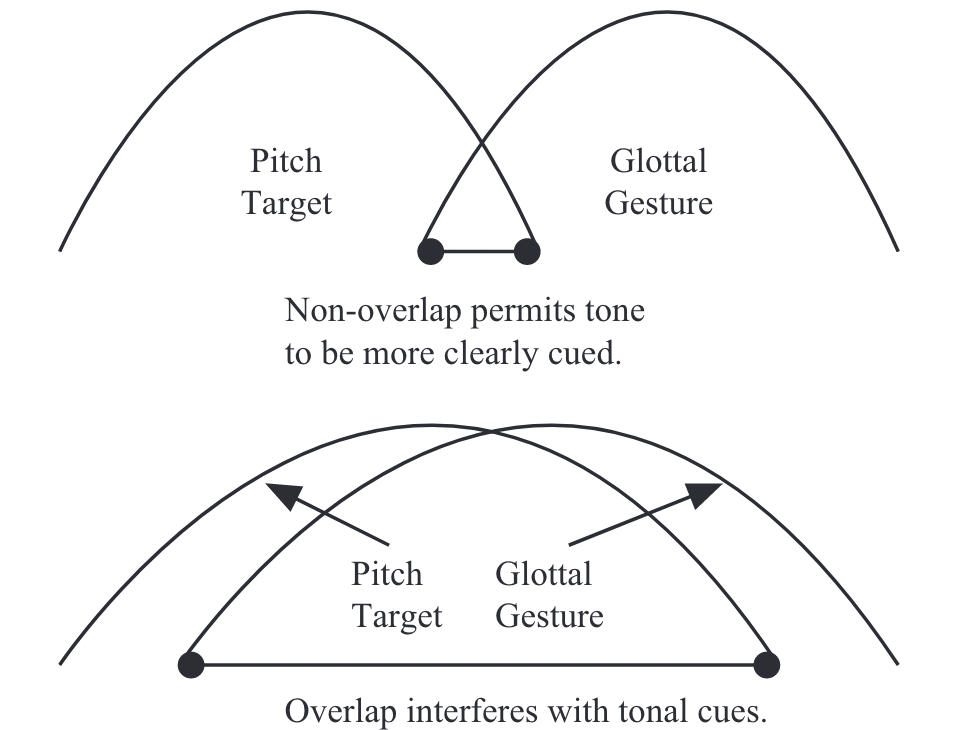
\includegraphics[width=.5\textwidth]{../Gestures.png}
	\caption{Representation taken from \citet{dicanioCoarticulationToneGlottal2012}.}
	\label{fig:GlottalGestures}
\end{figure}

Some work has been done into investigating this in other languages, most notably \posscitet{dicanioCoarticulationToneGlottal2012} investigation into glottals in Itunyoso Trique, which is also an Oto-Manguean language. \citeauthor{dicanioCoarticulationToneGlottal2012} in his study found that when the magnitude of coarticulation for glottal consonants occurs on the vowels there is a strong correlation between the magnitude of overlap and the amount of perturbation in the f0 signal. If, however, the degree of overlap was minor then the acoustic signal had little to no perturbation. These results were found by consulting the spectral tilt of the vowels with the f0 measures and performing a generalized linear mixed effects model with speaker treated as a random effect. 

Another study on Jalapa Mazatec \citep{garellekAcousticConsequencesPhonation2011} also investigated the interaction of tone and phonation. Jalapa Mazatec is a language with both contrastive tone and phonation and \citet{garellekAcousticConsequencesPhonation2011} validated the claims made by the LCH, in that tone and phonation seemed to be ordered with each other when it comes to at least one of the phonation types.

In testing the claims made by the LCH, this paper investigates the interaction of tone and phonation in the Northern Zapotec language of Santiago Laxopa Zapotec. This language is ideal for testing the viability of the LCH because of its use of both contrastive tone and phonation. The rest of the paper will provide a description of the language in Section~\ref{sec:SLZ} with special emphasis on the tone and phonation systems. Following this discussion on Santiago Laxopa Zapotec, this paper discusses an acoustic analysis of phonation modelled on \citet{espositoVariationContrastivePhonation2010,garellekAcousticConsequencesPhonation2011,dicanioCoarticulationToneGlottal2012} in Section~\ref{sec:Acoustics}.

%------------------------------------
\section{Santiago Laxopa Zapotec} \label{sec:SLZ}
%------------------------------------

Santiago Laxopa Zapotec (SLZ; \textit{Dilla'xhonh Laxup}) is a Northern Zapotec language spoken by approximately 1000 people in the municipality of Santiago Laxopa, Ixtlán District in the Sierra Norte of Oaxaca, Mexico \citep{adlerAcousticsPhonationTypes2016,adlerDerivationVerbInitiality2018,foleyForbiddenCliticClusters2018,foleyExtendingPersonCaseConstraint2020}. It is closely related to San Bartolomé Zoogocho Zapotec \citep{longDiccionarioZapotecoSan2005,sonnenscheinDescriptiveGrammarSan2005} and is mutually intelligible with this variety according to native speakers.  As is common among Zapotecan languages, SLZ distinguishes between lenis and fortis consonants \citep[e.g.,][]{nellisFortisLenisCajonos1980,jaegerFortisLenisQuestion1983,uchiharaFortisLenisGlides2016} and has a fairly standard five-vowel inventory. These contrasts and inventories can be seen in Table~\ref{tab:SLZcons} and Table~\ref{tab:SLZvowels}.


\begin{table}[!h]
	\centering
	\caption{Consonant inventory for Santiago Laxopa Zapotec}
	\label{tab:SLZcons}
	\fittable{
	 \begin{tabular}{llcccccccc}
	  \lsptoprule
		  &  & bilabial & alveolar  & retroflex & alveo- & palatal &velar &labio-  &  uvular \\
		 &&&&& palatal &&&velar& \\
	  \midrule
		nasal    	& lenis   &	   & n  & & & & & & \\
					& fortis  &	mː & nː & & & & & & \\
		stop 		& lenis   & b  & d  & & & & g & gʷ & \\
					   & fortis  & p  & t  & & & & k & kʷ & \\
		fricative   & lenis   &    & z  & ʐ\textasciitilde ɽ & ʒ & ç & &  & ʁ\textasciitilde χ \\
					   & fortis  &    & s  & ʂ & ʃ & & & & \\
		  affricate 	& lenis   &    & d͡z & & & & & & \\
					  & fortis  &    & t͡s & & t͡ʃ & & & & \\
		lateral  	& lenis   &    & l\textasciitilde ɾ & & & & & & \\
					& fortis  &    & lː & & & & & & \\
		trill		& 		  &    & r & & &  & &  & \\ 			
		approximate & 		  &    & & & & j & & w & \\ 
	  \lspbottomrule
	 \end{tabular}
	 }
	\end{table}

	\begin{table}[!h]
		\centering
		\caption{Vowels inventory in Santiago Laxopa Zapotec.}
		\label{tab:SLZvowels}
		 \begin{tabular}{lccc}
		  \lsptoprule
					&  front& central  & back \\
		  \midrule
			high   	&  i  &     &   u \\
			mid    	&  e  &   	& 	o \\
			low   	&     &  a 	&	  \\
		  \lspbottomrule
		 \end{tabular}
		\end{table}
		
In addition to the contrasts in both consonants and vowels, SLZ additionally has a phonation and tonal contrast. I will first talk about the tonal contrasts in Section~\ref{sec:Tone} followed by the tonal phonation in Section~\ref{sec:Phonation}.

%------------------------------------
\subsection{Tone in SLZ} \label{sec:Tone}
%------------------------------------

As is common among Oto-Manguean languages, SLZ is a tonal languages \citep{suarezMesoamericanIndianLanguages1983,campbellMesoAmericaLinguisticArea1986,silvermanLaryngealComplexityOtomanguean1997,campbellOtomangueanHistoricalLinguistics2017a,campbellOtomangueanHistoricalLinguistics2017}. In SLZ there are five surface tones which appear on a syllable. Following other papers on SLZ, I am representing the tone using Pike's numbers \citep[e.g.][]{sichelFeaturalLifeNominals2020}. Pike's numbers are commonly used in describing Mesoamerican tone systems and has its origins in \posscitet{pikeToneLanguagesTechnique1948} work with Mixtec. A good summary of this system and its comparisons to other tone marking systems is given in \citet{weePhonologicalTone2019}. Pike's numbers represent the highest tone with the number 1 and then each subsequent tonal level is represented with the next number until all levels have been assigned. In the case of a language with three distinct levels the number 1 represents the highest tone, the number 2 represents the mid tone, and finally the number 3 represents the lowest tone. Additionally, these different numbers can be combined to represent the different contour tones that exist in the language, for example 21 representing a tone that starts at the mid level and then increases its pitch to high. 


\begin{table}[!h]
	\centering
	\caption{Examples of the five tonal patterns observed in the Santiago Laxopa Zapotec words.}
	\label{tab:tones}
	 \begin{tabular}{lllll}
	  \lsptoprule
					  % &	 Diacritic  & Example & Transcription \\
	  High   	&  a¹  &  \textit{xha}   &  [ ʐa¹ ] & `clothing.\textsc{poss}'\\
		Mid    	&  a²  &  \textit{lhill} 	& [ ɾiʒ² ] & `house.\textsc{poss}' \\
		Low   	&  a³  &  \textit{yu'} 	&	 [ juˀ³ ] & `earth'\\
		Rising	&  a²¹  &  \textit{yu'u} 	&	[ juˀu²¹ ] & `quicklime (Sp. cal)' \\
		Falling &  a¹³  &  \textit{yu'u}  &	[juˀu¹³] &	`house' \\
	  \lspbottomrule
	 \end{tabular}
\end{table}

\begin{figure}[!ht]
	\centering
	\includegraphics[width=0.9\textwidth]{../FSRTonePlot.png}
	\label{fig:FSRTonePlot}
	\caption{Tonal contrasts for FSR averaged and time normalized. Each line in this graph represents the average of approximately 10 syllables for each tonal pattern. }
\end{figure}

\begin{figure}[!ht]
	\centering
	\includegraphics[width=0.9\textwidth]{../RDTonePlot.png}
	\label{fig:RDTonePlot}
	\caption{Tonal contrasts for RD averaged and time normalized. Each line in this graph represents the average of approximately 10 syllables for each tonal pattern.}
\end{figure}

Following discussion from \citet{brinkerhoffTonalPatternsTheir2022} these tones appear to be limited in their distribution. It is true that all five patterns can surface on a syllable but there is a restriction in what tonal patterns are allowed to surface on words that are larger than bimoraic. The patterns that we observe on bimoraic nominals are: HL, MH, and LL.
% \begin{figure}[!ht]
% 	\centering
% 	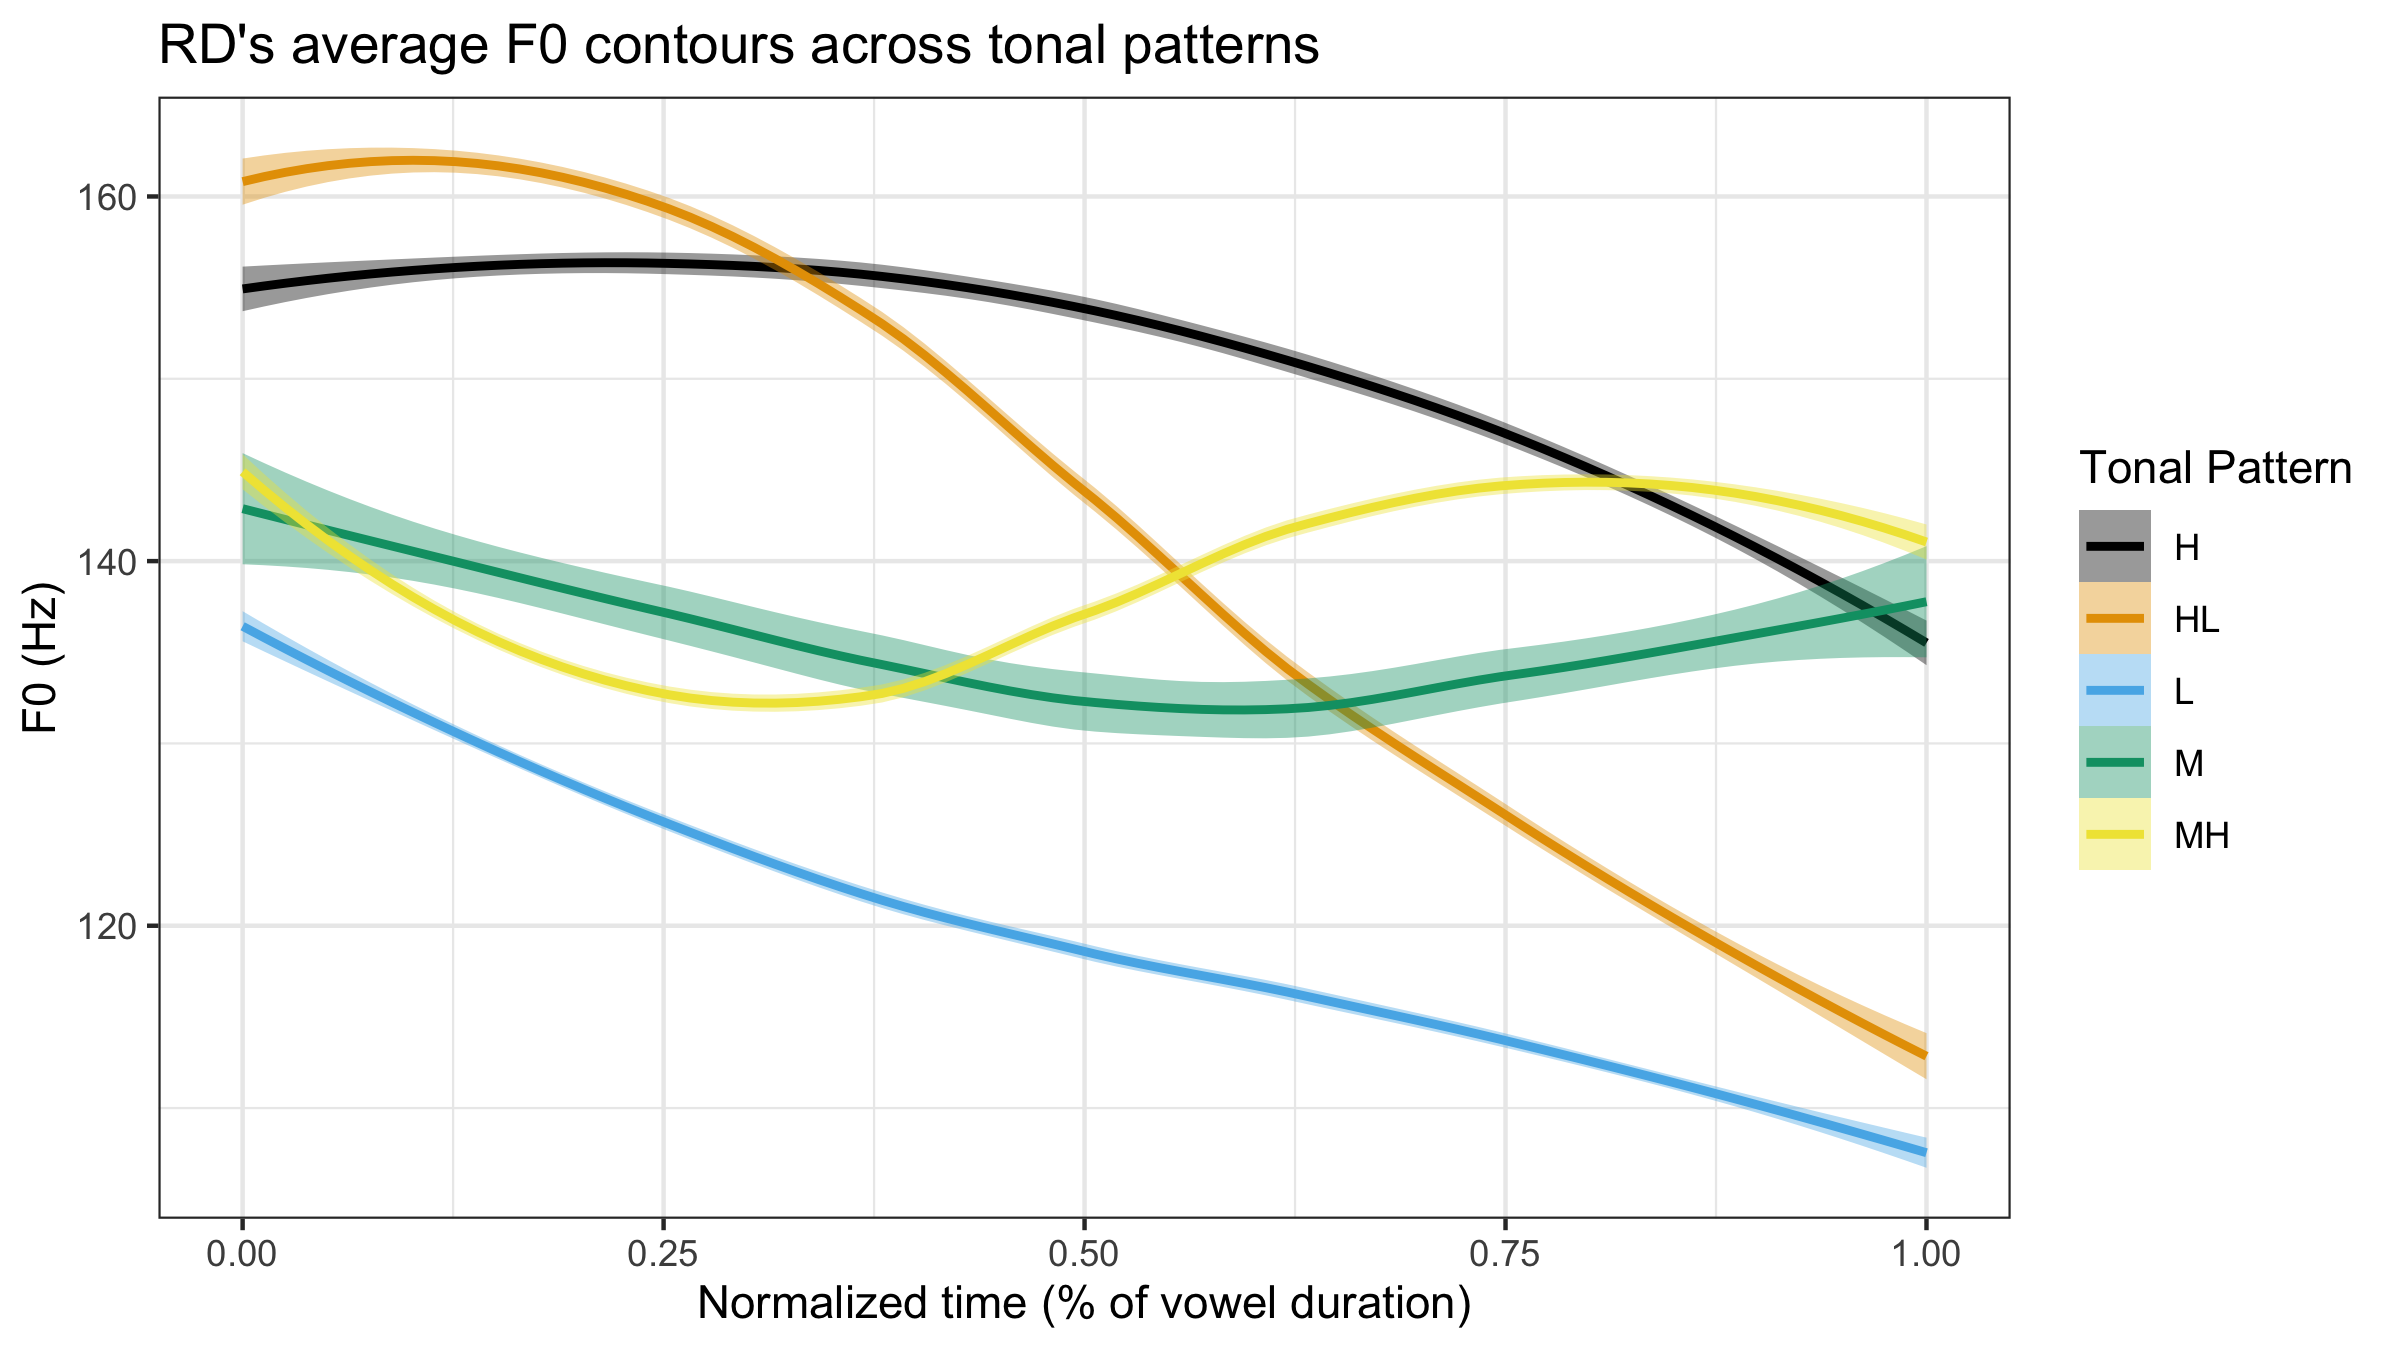
\includegraphics[width=0.9\textwidth]{../JoinTonePlot.png}
% 	\label{fig:LAMNetwork}
% 	\caption{Tonal contrasts for FSR and RD normalized for f0 and time.}
% \end{figure}

%------------------------------------
\subsection{Phonation in SLZ} \label{sec:Phonation}
%------------------------------------

Among Zapotecan languages it is quite common for languages to make use of contrastive phonation \citep[e.g.,][]{avelinobecerraTopicsYalalagZapotec2004,longDiccionarioZapotecoSan2005,avelinoAcousticElectroglottographicAnalyses2010,lopeznicolasEstudiosFonologiaGramatica2016,chavez-peonInteractionMetricalStructure2010}. 
SLZ, in addition to the five vowel qualities, has four contrastive phonation types which are: modal, breathy, checked, and laryngealized. These contrasts are exemplified in the minimal quadruple in (\ref{ex:YA}). In representing the checked and laryngealized vowels, I follow the same procedure as other authors (e.g., \citet{avelinoAcousticElectroglottographicAnalyses2010, uchiharaToneRegistrogenesisQuiavini2016}) in representing the `glottal stop' element as a superscripted glottal stop in the IPA transcription (i.e., [aˀ]). This is primarily done as a way of standardizing the variable pronunciation of the glottal element in Zapotec ranging from a full glottal stop (i.e., [aʔ]) to creaky voice on a portion of the vowel (i.e., [aa̰]).  

\ea \label{ex:YA} Four-way minimal phonation contrast
	\ea \textit{ya} [ja³]	`bell'
	\ex \textit{yah}  [ja̤³] `metal/rifle'
	\ex \textit{ya'}  [jaˀ³]  `pound'
	\ex \textit{ya'a}  [jaˀa³]  `market'
	\z 
\z 

Breathy phonation on vowels is characterized by a raspy quality throughout the whole vowel or a portion toward the end of the vowel, see Figure~\ref{fig:BreathyVowel}. 

\begin{figure}[!h]
	\centering
	% [INSERT YAH SPECTROGRAM AND WAVEFORM]
	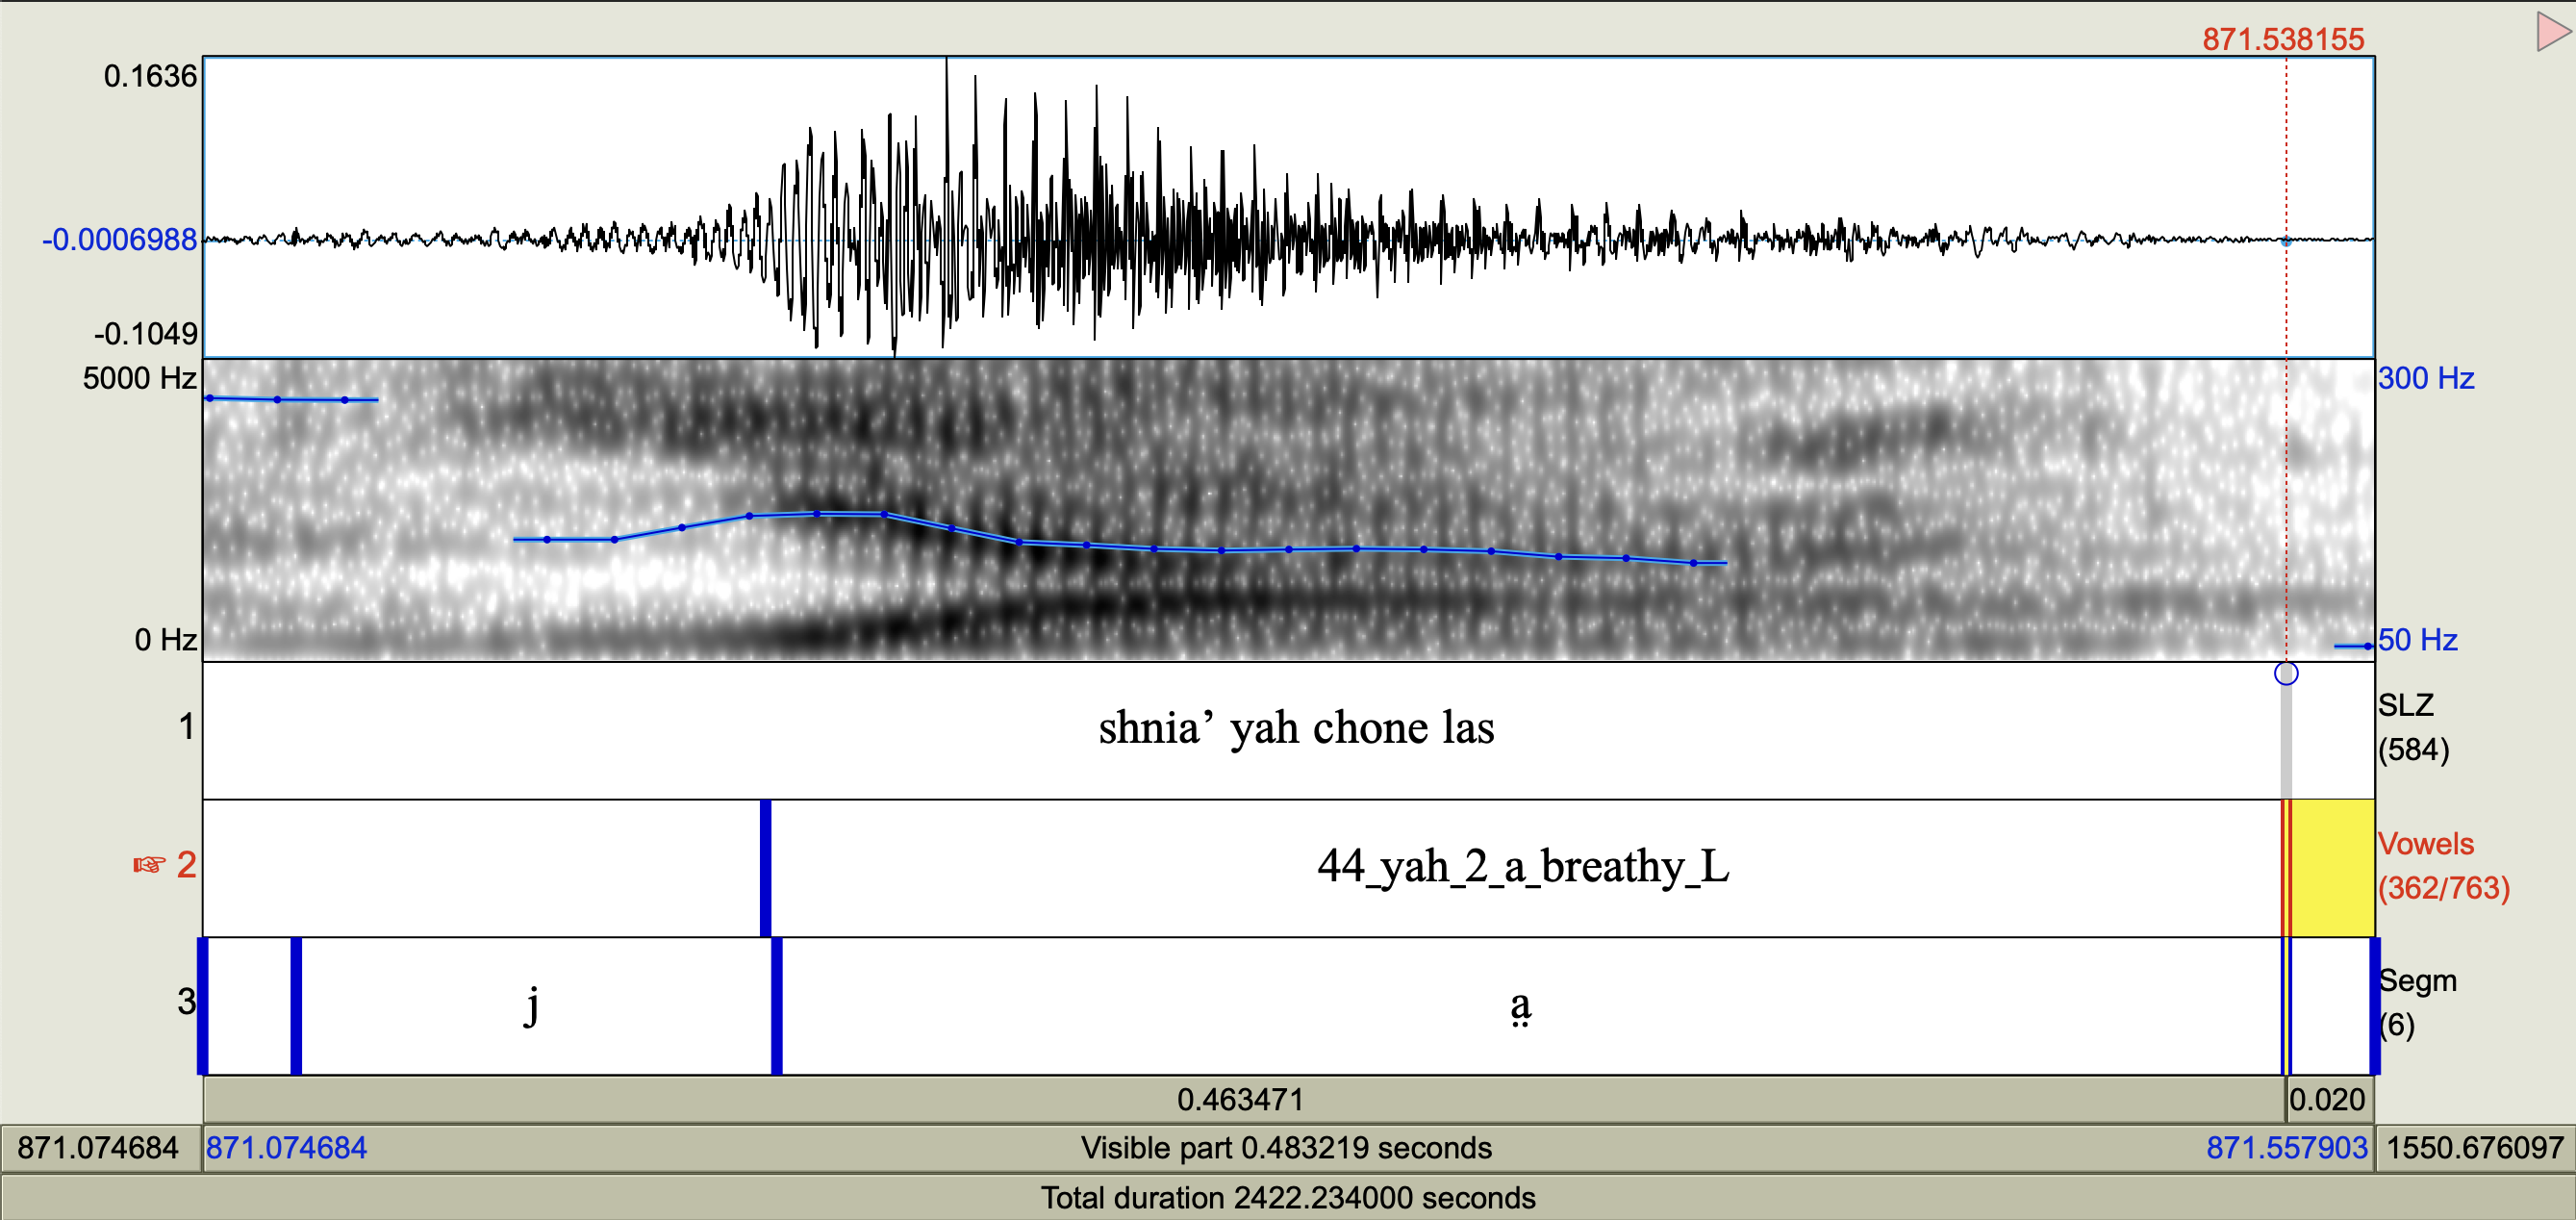
\includegraphics[width=0.9\textwidth]{../yah.png}
	\caption{Breathy vowel in the word \textit{yah} `metal/rifle'}
	\label{fig:BreathyVowel}
\end{figure}

Checked vowels on the other hand are characterized by an abrupt glottal closure which cuts the vowel short. This phonation is sometimes only realized as a very short period of creakiness at the end of the vowel, see Figure~\ref{fig:CheckedVowel}.  

\begin{figure}[!h]
	\centering
	[INSERT YA' SPECTROGRAM AND WAVEFORM]
	% 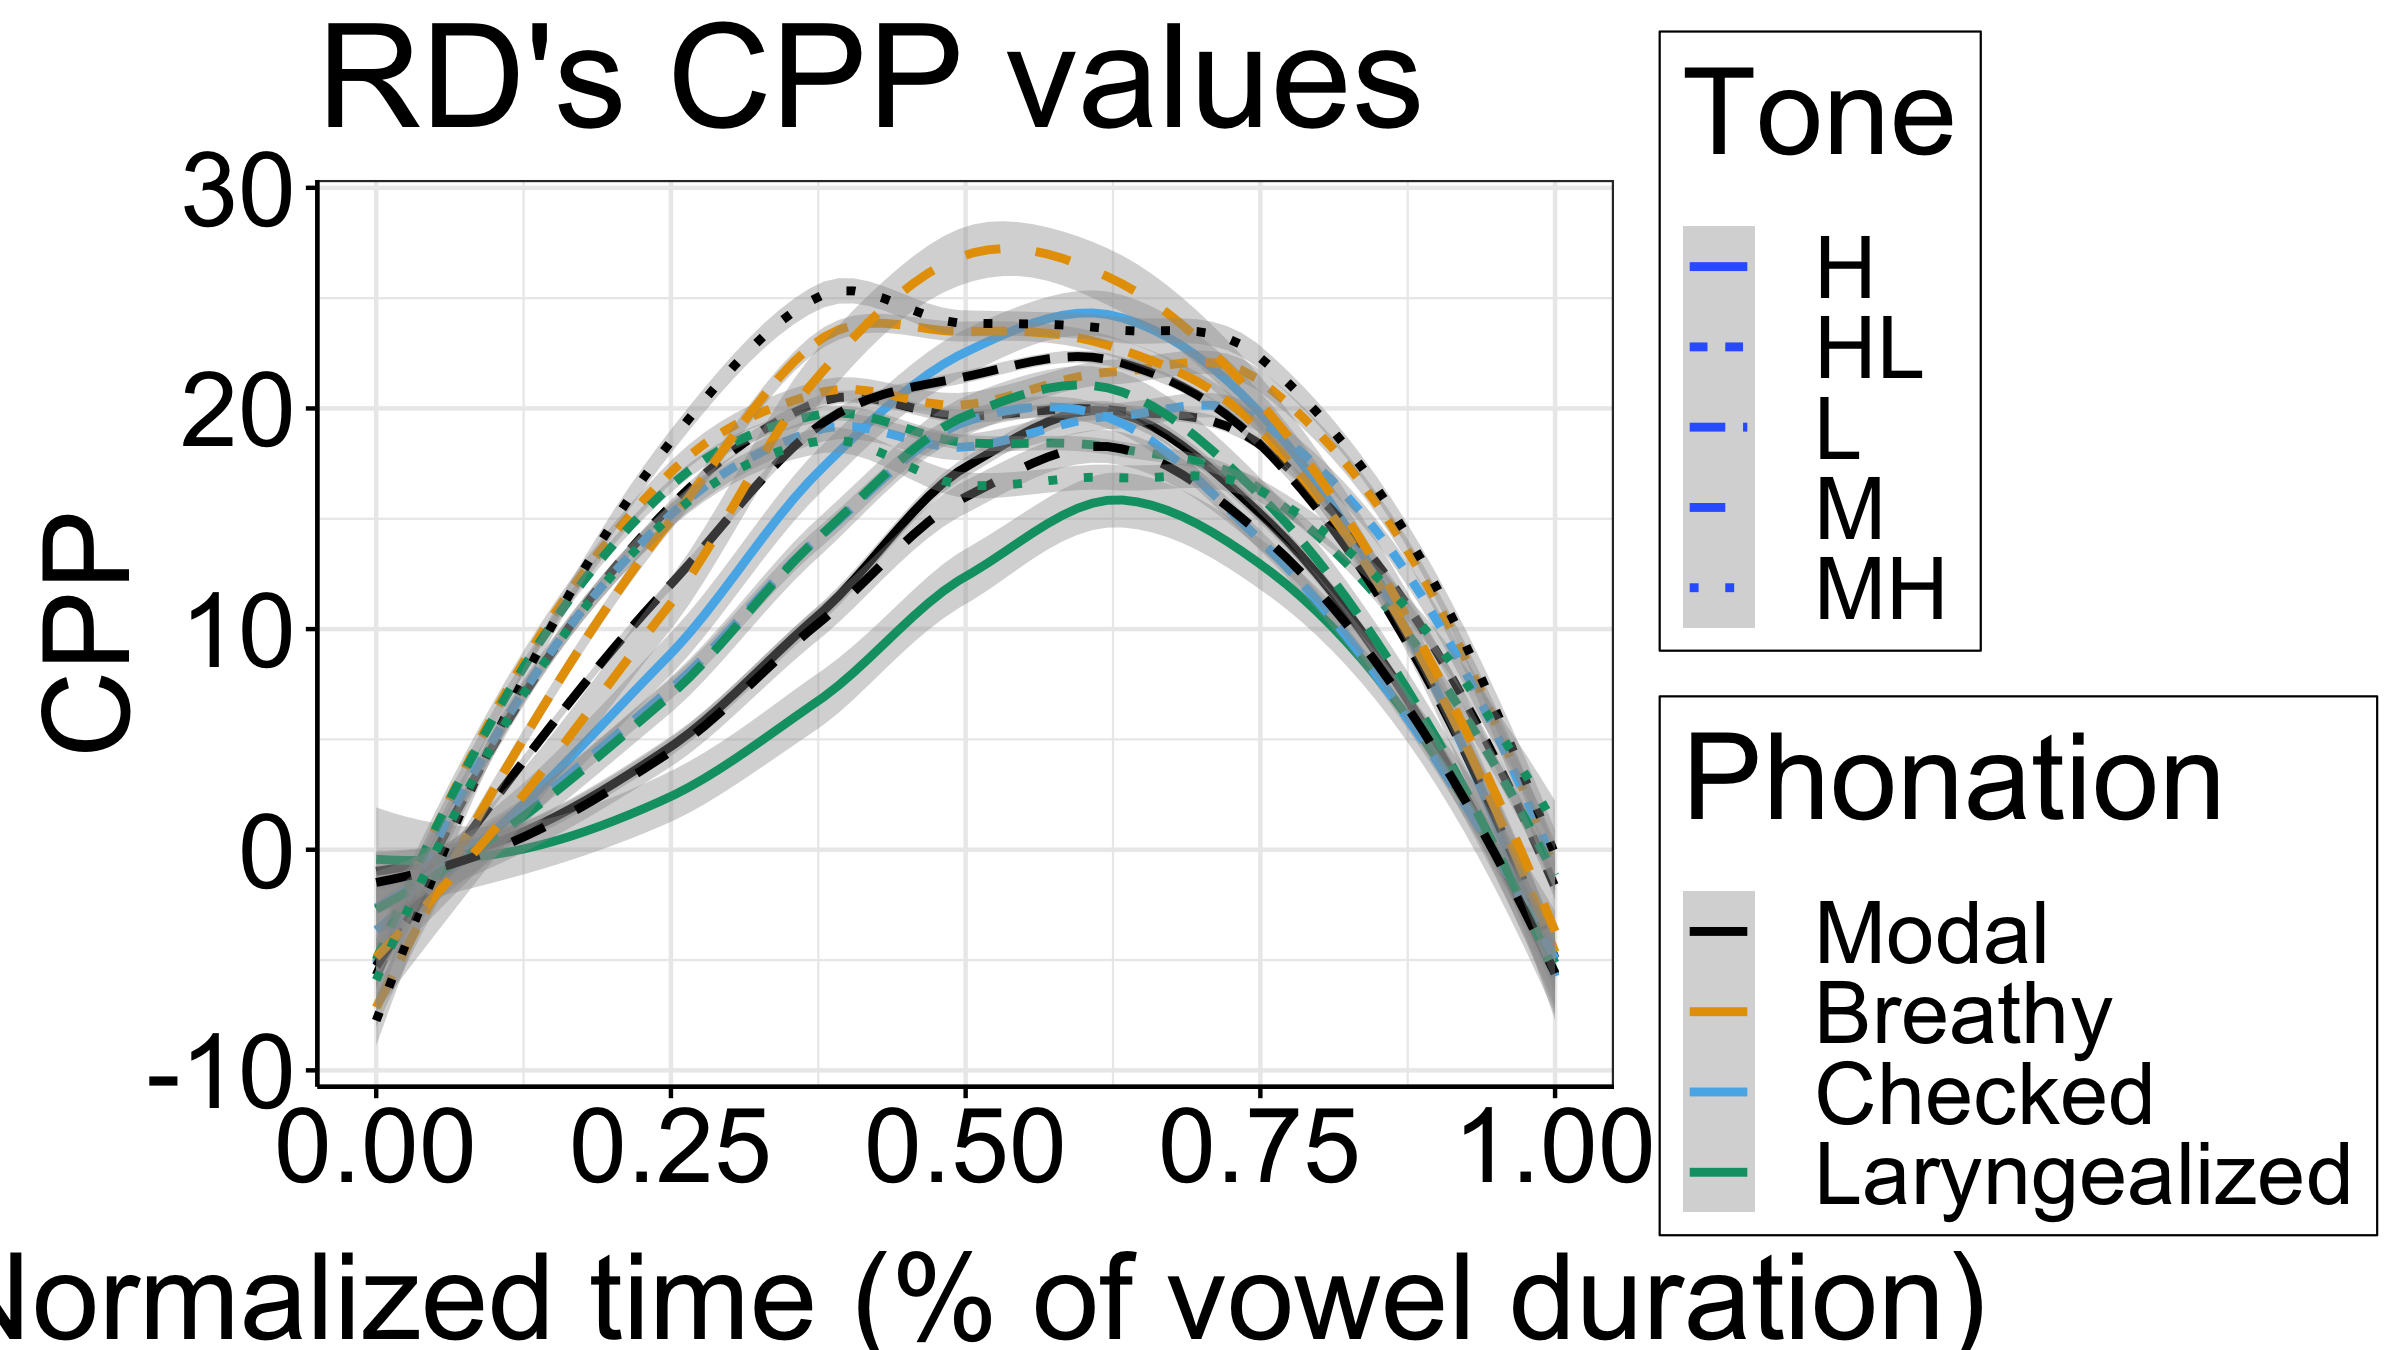
\includegraphics[width=0.9\textwidth]{../RDCPP_line.png}
	\caption{Breathy vowel in the word \textit{ya'} `pound'}
	\label{fig:CheckedVowel}
\end{figure}

Laryngealized vowels are quite common in Zapotecan languages and have received a wide number of different names. Previous descriptions have used terms such as broken, rearticulated, interrupted, and creaky \citep{longDiccionarioZapotecoSan2005,avelinobecerraTopicsYalalagZapotec2004,avelinoAcousticElectroglottographicAnalyses2010,sonnenscheinDescriptiveGrammarSan2005,adlerAcousticsPhonationTypes2016}. In order to avoid confusion, I will use the term laryngealized following \citet{avelinoAcousticElectroglottographicAnalyses2010}. In addition to a wide number of different names these vowels also exhibit a wide range of allophones. 

\citet{avelinoAcousticElectroglottographicAnalyses2010} found in the closely realted Yalálag Zapotec that among his consultants there were at least four different pronunciations as seen in Table~\ref{tab:laryngeal}. 
\begin{table}[!h]
	\centering
	\caption{Layngealized Vowels in Yalálag Zapotec}
	\label{tab:laryngeal}
	 \begin{tabular}{ll}
	\lsptoprule
	/VˀV/	&  [VʔV]  \\
			&  [VV̰V]   \\
			&  [VV̰ːV̆]  \\
			&  [VV̰V̰]	\\
	\lspbottomrule
	\end{tabular}
\end{table}
In SLZ, each of the consulted language experts would produce this vowel differently. One consultant would do rearticulation, where there is a full glottal stop in the middle of the vowel, or creaky voice. This alternation seemed to be in free variation but there was a greater tendency to creak in low toned words, such as \textit{xa'ag} [ʂa̰ːg] `topil'\footnote{A topil is a type of government office in traditional Oaxacan communities somewhat akin to a sheriff. }, see Figure~\ref{fig:FSRLaryngeal} for a comparison between this consultant's pronunciation of the laryngealized vowels.

\begin{figure}[!h]
	\centering
	\begin{subfigure}{.5\textwidth}
		\centering
		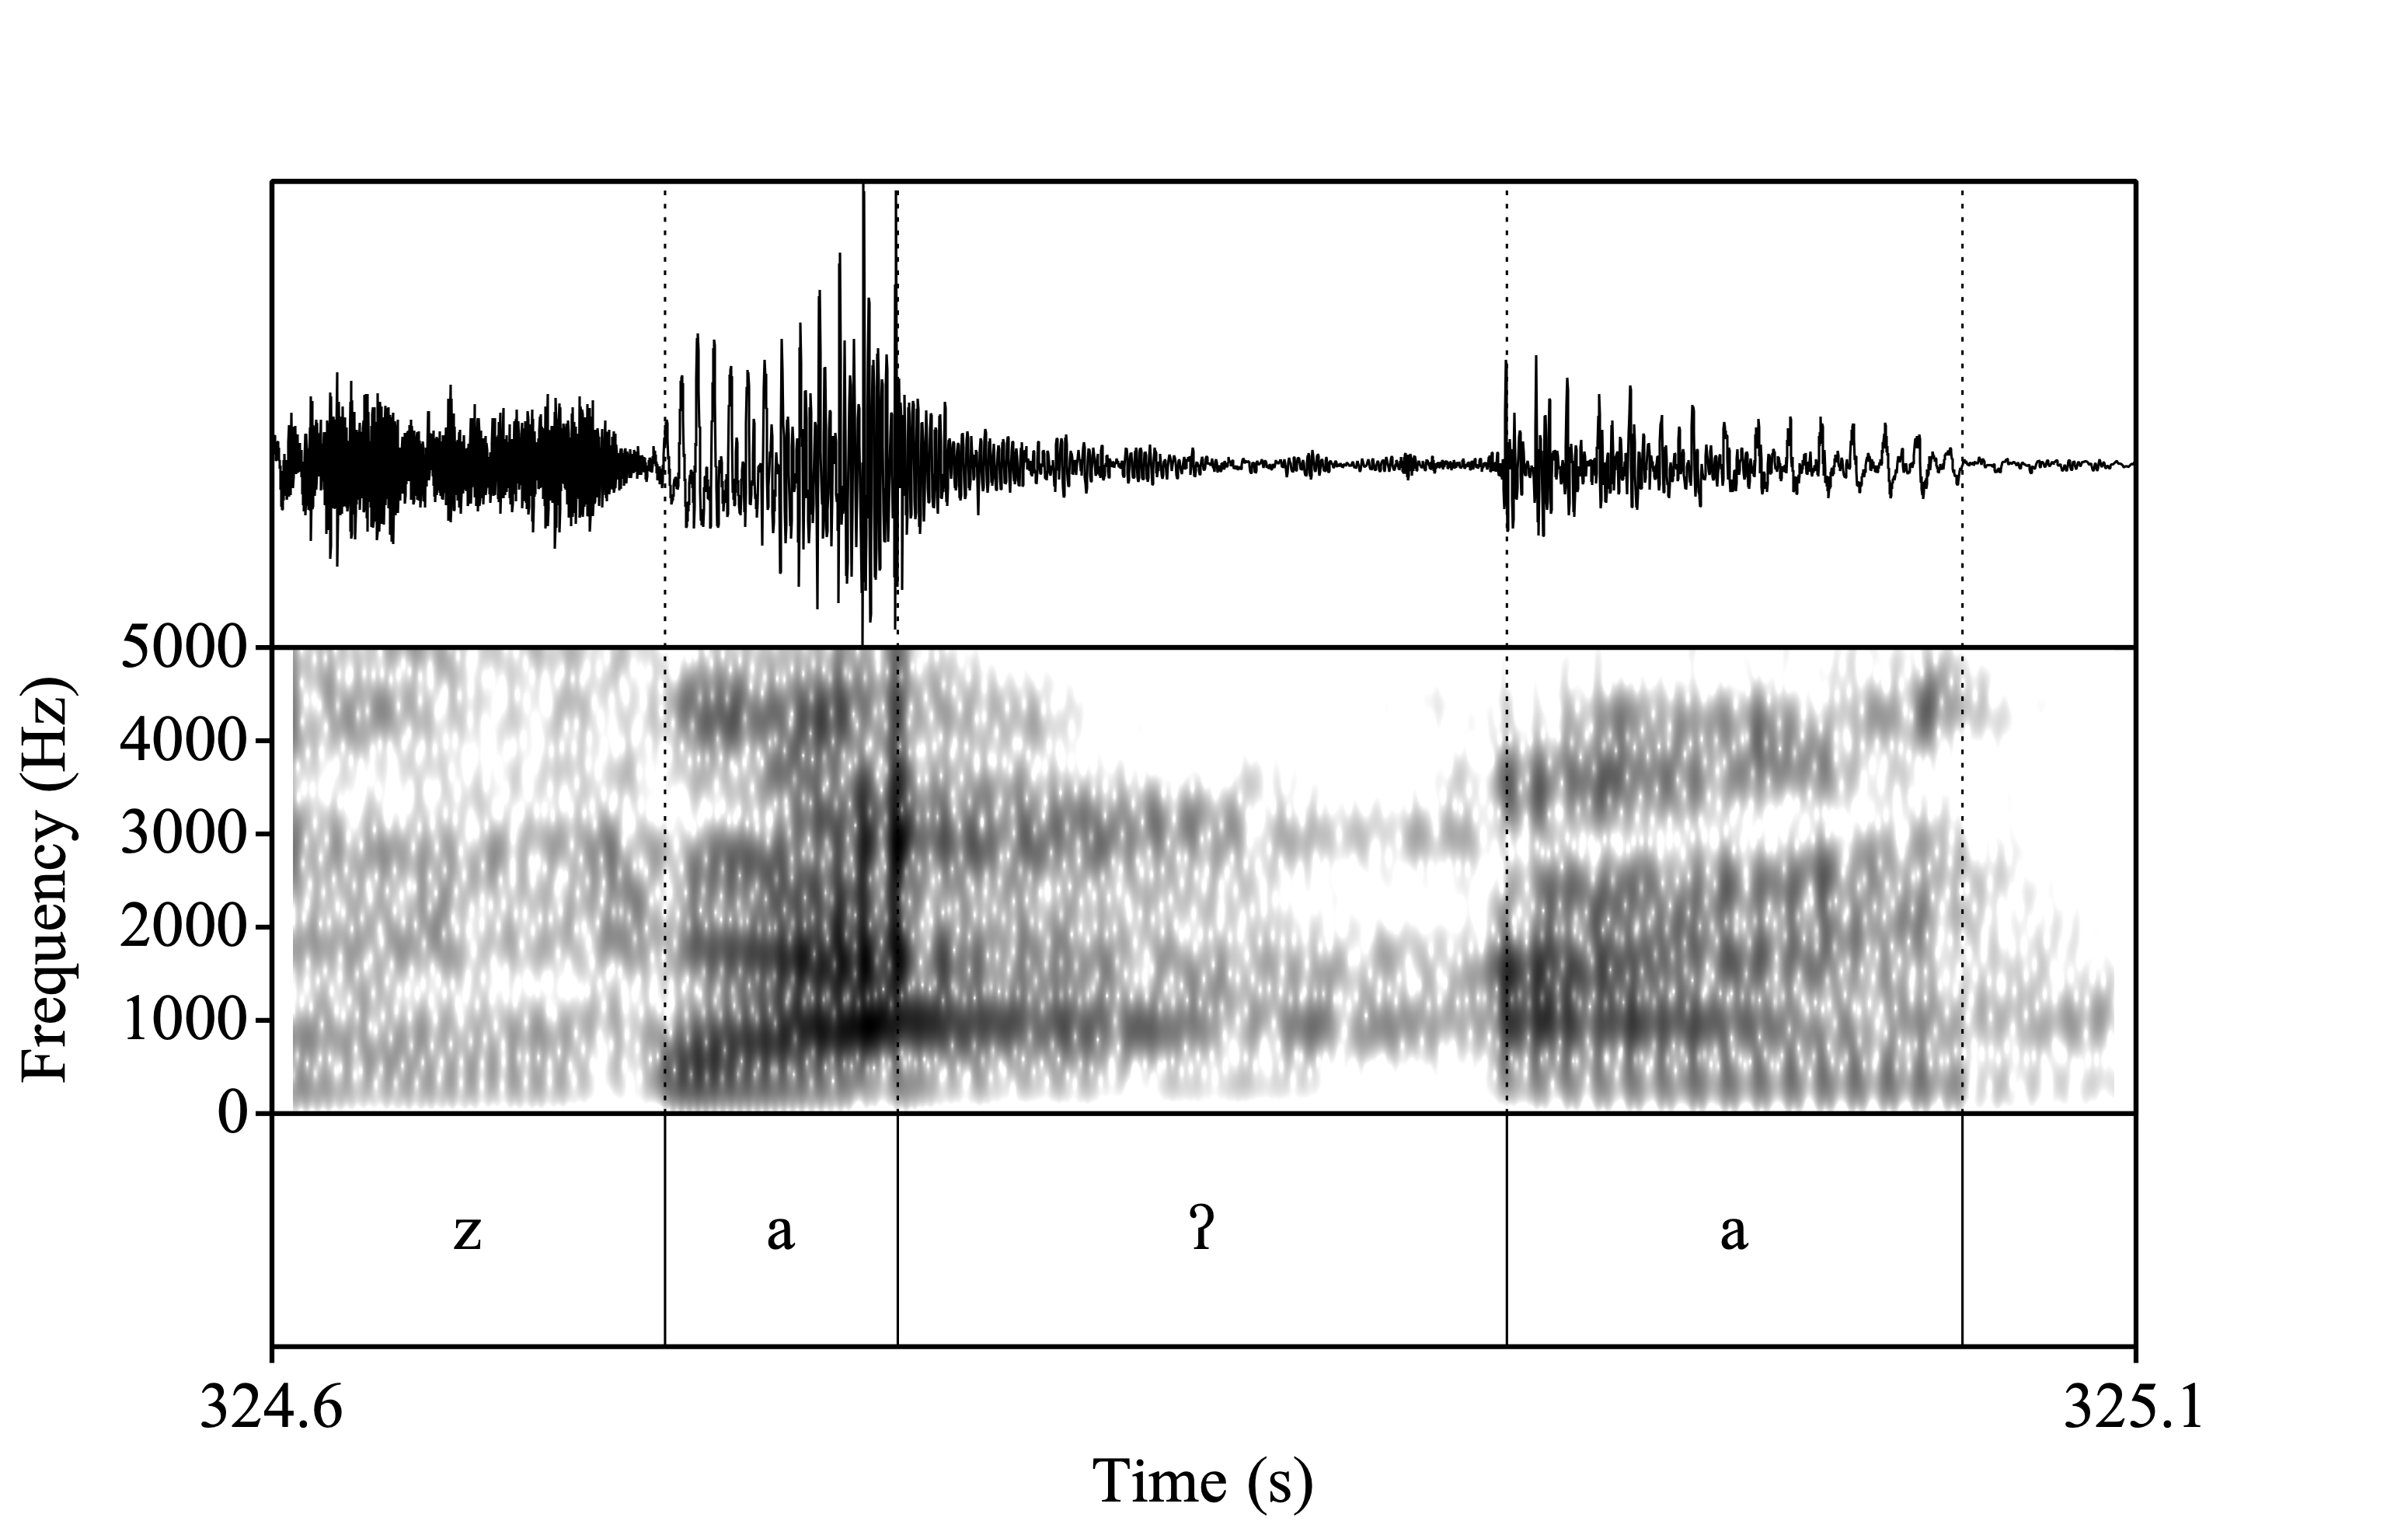
\includegraphics[width=\linewidth]{../za'a.png}
		\caption{\textit{za'a} `corncob'}
		\label{fig:za'a}
	\end{subfigure}%
	\begin{subfigure}{.5\textwidth}
		\centering
		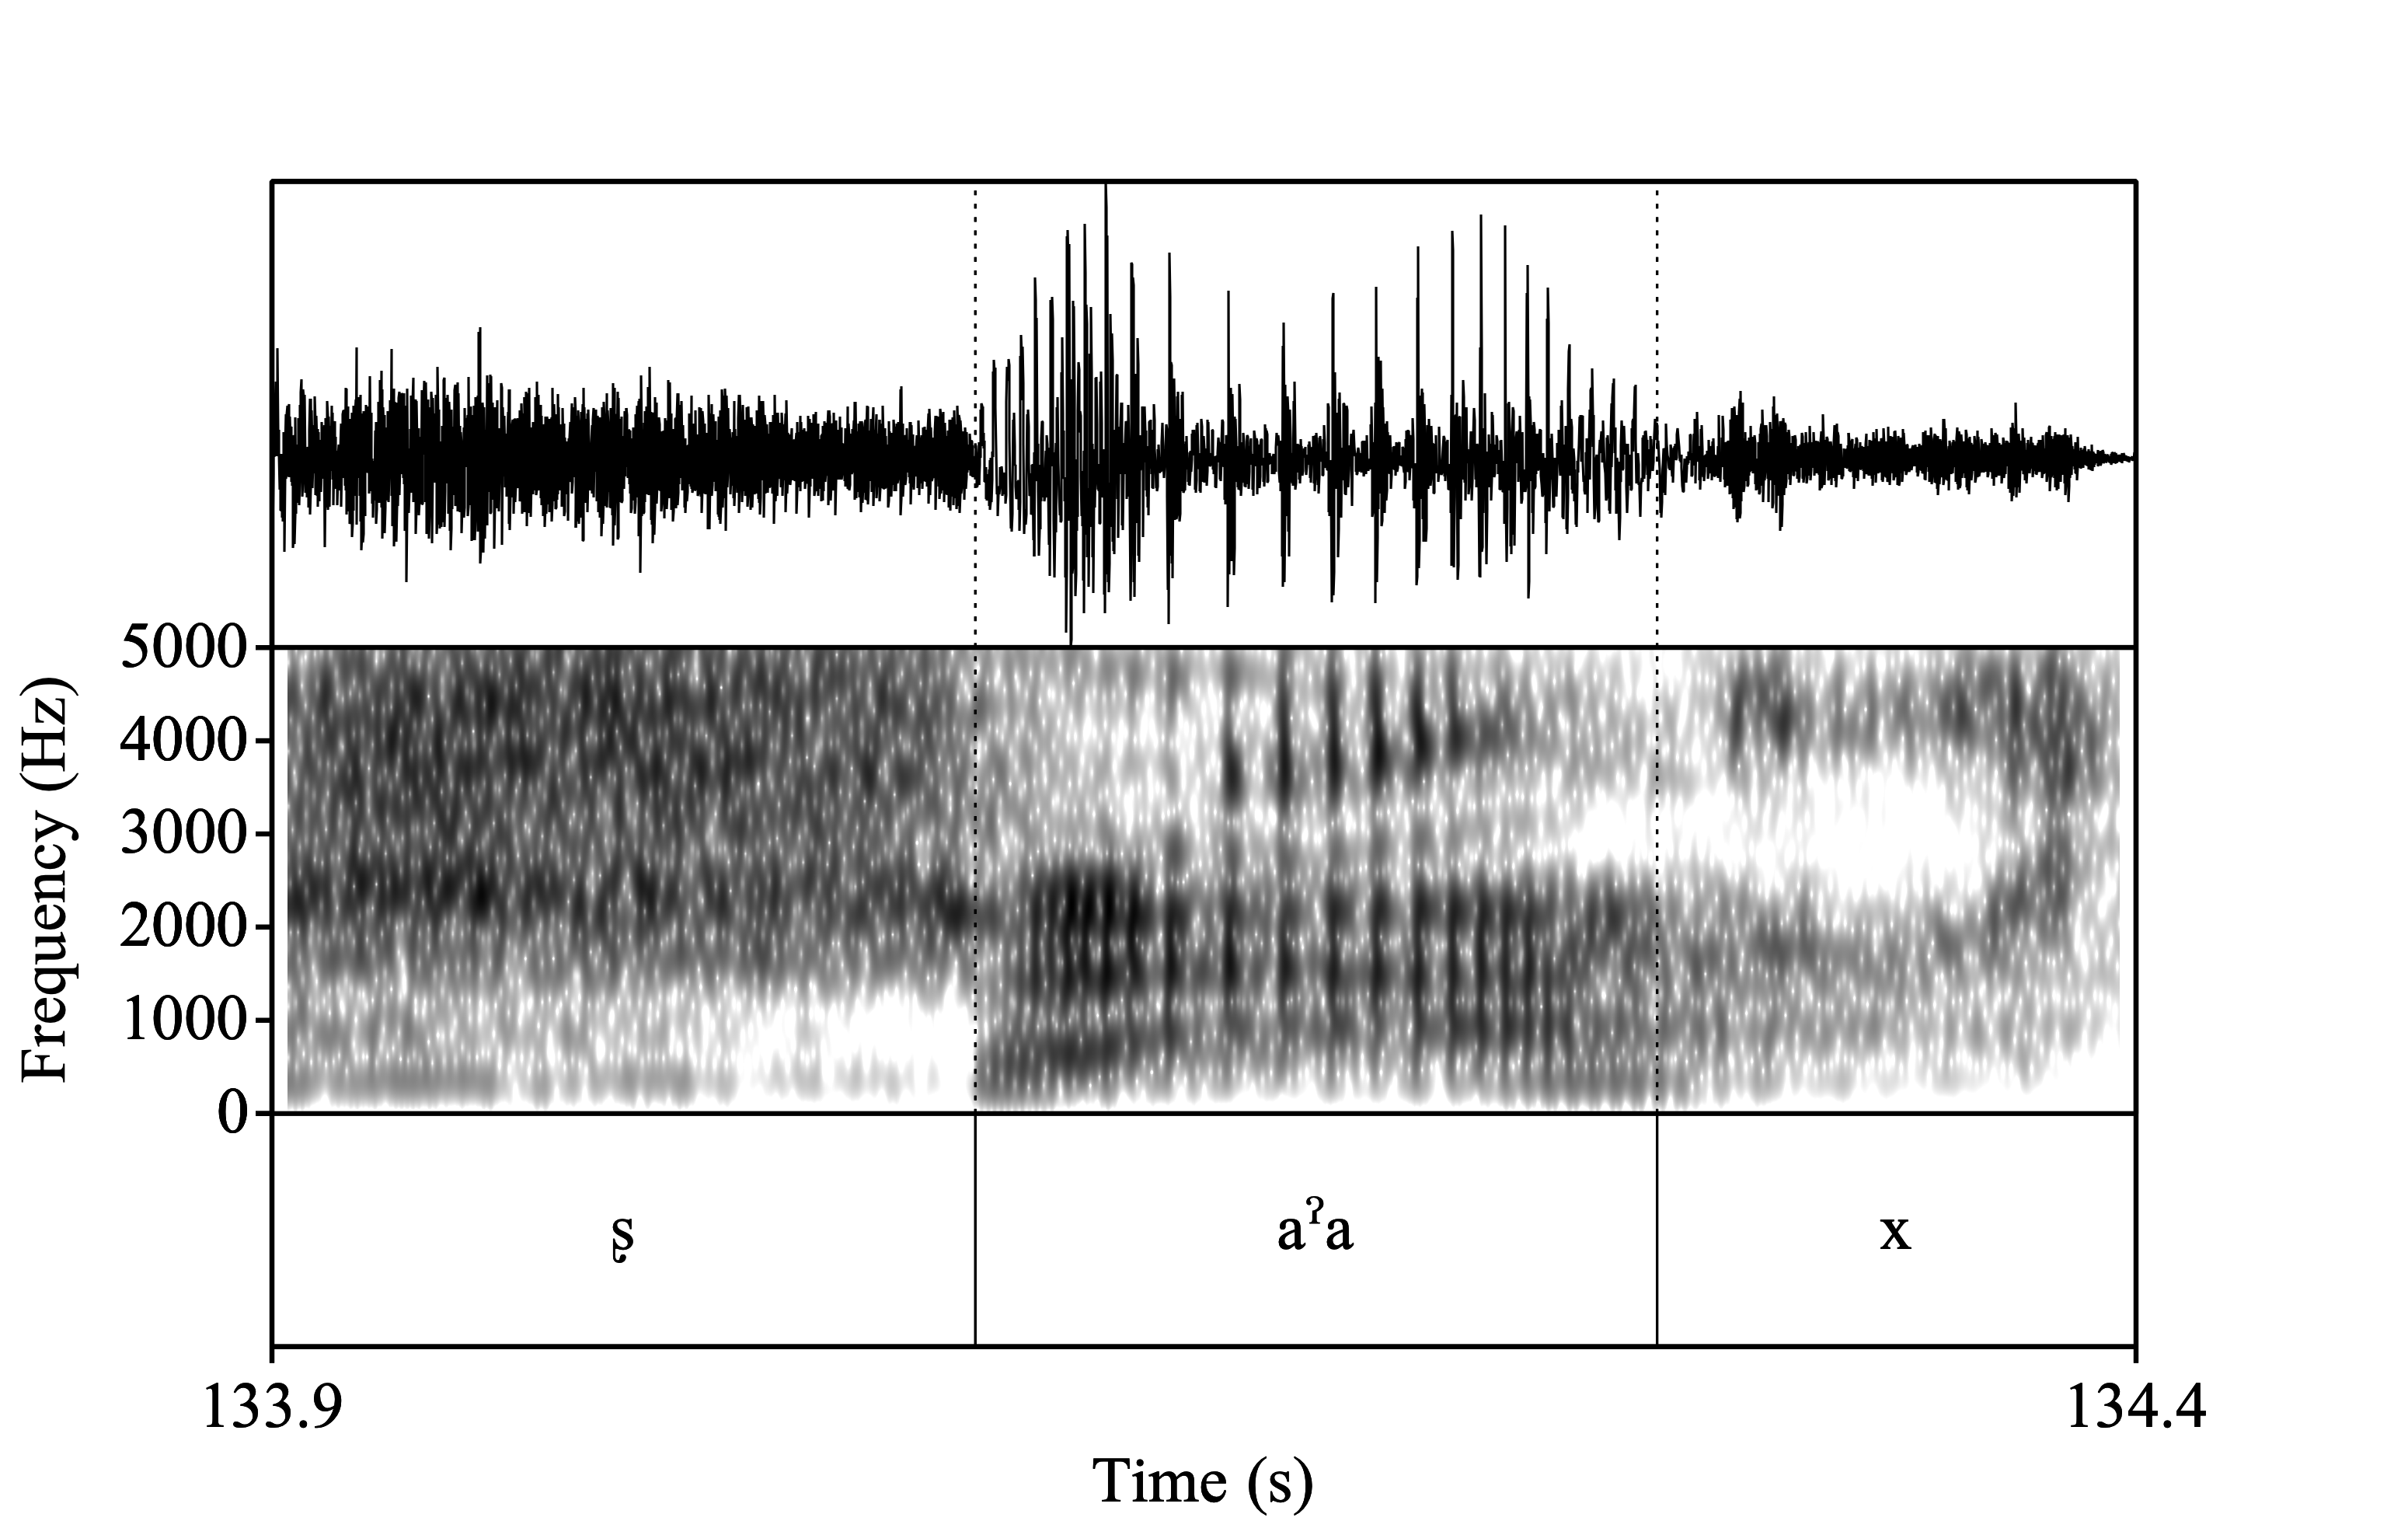
\includegraphics[width=\linewidth]{../xa'ag.png}
		\caption{\textit{xa'ag} `topil'}
		\label{fig:xa'ag}
	\end{subfigure}	
	\caption{Comparison of FSR's laryngealized vowels in \textit{za'a} `corncob' and \textit{xa'ag} `topil'}
	\label{fig:FSRLaryngeal}
\end{figure}

The other consultant only ever produces creaky voice for these vowels regardless of the tone with the word. During one of the elicitation sessions, we conducted a perceptual check that these were in fact the same vowels and both consultants reliably identified the words and produced laryngealized vowels according to their own idiosyncrasies. However, a more detailed perception study is beyond the scope of this paper. 
\begin{figure}[!h]
	\centering
	[INSERT SIDE BY SIDE SPECTROGRAMS]

	\caption{Comparison of RD's laryngealized vowels in \textit{za'a} `corncob' and \textit{xa'ag} `topil'}
	\label{fig:RDLaryngeal}
\end{figure}

%------------------------------------
\section{Interaction of Tone and Phonation} \label{sec:Interaction}
%------------------------------------

Most previous work on the interaction of tone has been focused on the languages of East and Southeast Asia 
\citep[e.g.,][]{masicaDefiningLinguisticArea1976,thurgoodVietnameseTonogenesisRevising2002,yipTone2002,enfieldArealLinguisticsMainland2005,michaudComplexTonesEast2012,brunelleTonePhonationSoutheast2016}. 
What has been found in these descriptions is that certain tones and phonations are codependent (i.e., only occur with each other). For example \citet{smalleyProblemsConsonantsTone1976} and \citet{ratliffMeaningfulToneStudy1992} both describe White Hmong's \textit{-g} tone as being a mid-low tone with breathy phonation and Mandarin's tone 3 is often associated with creaky phonation \citep{hockettPeipingPhonology1947}. \citet{brunelleTonePerceptionNorthern2009} found that creaky phonaiton plays an important role in the production of certain tones. Additionally, work on S'gaw Karen has found that two tones are only differentiated by the presence of some form of non-modal phonation (Boehm p.c.). 

However, there has been some observations–especially in Mesoamerica–that tone and phonation can co-vary \citep[e.g,][]{silvermanLaryngealComplexityOtomanguean1997,garellekAcousticConsequencesPhonation2011}. This means that tone can independently occur with any phonation type. This has also been extensively described in multiple Zapotecan languages \citep[e.g.,][]{,avelinobecerraTopicsYalalagZapotec2004,avelinoAcousticElectroglottographicAnalyses2010, chavez-peonInteractionMetricalStructure2010, campbellZenzontepecChatinoAspect2011,villardPhonologyMorphologyZacatepec2015, lopeznicolasEstudiosFonologiaGramatica2016}

\citet{chavez-peonInteractionMetricalStructure2010} has a detailed description of the tone and phonation interactions in San Lucas Quiaviní Zapotec (SLQZ), a central valley variety of Zapotec. The distribution of tone and phonation is found in Table~\ref{tab:SLQZ}. We see that in SLQZ, that both low and falling tone have the full range of possible combinations. However, we see gaps in the high tone for breathy and rising tone can only occur with modal phonation. 

\begin{table}[!ht]
	\centering
	\caption{SLQZ tone and phonation interactions \citep{chavez-peonInteractionMetricalStructure2010}.}
	\label{tab:SLQZ}
	 \begin{tabular}{lcccc}
	  \lsptoprule
					  &	 \textbf{Modal}  & \textbf{Breathy} & \textbf{Creaky} & \textbf{Interrupted} \\
		  High	& ✔︎ & -- & ✔︎ & ✔︎ \\
		  Low & ✔︎ & ✔︎ & ✔︎ & ✔︎ \\
		  Falling & ✔︎ & ✔︎ & ✔︎ & ✔︎ \\
		  Rising & ✔︎ & -- & -- & -- \\
	  \lspbottomrule
	 \end{tabular}
\end{table}

Based on elicitation data collected from 2020-2022, SLZ has a more expansive distribution of tone and phonation when compared to SLQZ but seems to be very similar to other Northern Zapotec varities \citep[e.g.,][]{avelinobecerraTopicsYalalagZapotec2004}. The distribution of SLZ tonal and phonation interactions are given in Table~\ref{tab:ToneVoiceQuality} for the number of tokens that were analyzed. 
\begin{table}[!h]
	\caption{Number of tokens analyzed in this paper for each interaction of tone and phonation.}
	\label{tab:ToneVoiceQuality}
	\centering

	\begin{tabular}{lcccc}
	\lsptoprule
		& \textbf{Modal} & \textbf{Breathy} & \textbf{Checked} & \textbf{Laryngealized} \\
	\hline
	High		& 12 & -- & 5	& 3 \\
	Mid			& 7 & 1  & 2	& 1 \\
	Low			& 17 & 5  & 9	& 3 \\
	High-Low	& 9 & 1  & 2	& 1 \\
	Mid-High	& 1	 & 1  & --	& 1 \\
	\lspbottomrule
	\end{tabular}
\end{table}

One of the striking things in this is the lack of high tone with breathy phonation. This gap is interesting because of the long time association of high pitch with breathiness \citep[a good overview–of this association and other phoantion types–is found in][]{eslingVoiceQualityLaryngeal2019}. This gap of breathy phonation and high tone is quite common across the Zapotecan languages (Campbell p.c.). In the case of breathy phonation in SLQZ, \citet{uchiharaToneRegistrogenesisQuiavini2016} offers some convincing evidence that the phonation originated in syllables with low tone and then spread to other tones via analogy. 

%------------------------------------
\section{Acoustic investigation into the phonation} \label{sec:Acoustics}
%------------------------------------

One of the primary ways to measure and investigate phonation is using spectral measures. The most frequent type of measurement is spectral-tilt. Spectral-tilt measurements are conducted by comparing the relative amplitude of different harmonics in the acoustic signals, which has primarily been the difference in the relative amplitude of the first and second harmonics. Other measurements make use of higher harmonics which are closest to the different formants, see Figure~\ref{fig:Harmonics}. These spectral-tilt measurements have been found to be particularly useful in languages such as Green Hmong \citep{huffmanMeasuresPhonationType1987,andruskiPhonationTypesProduction2000} and Jalapa Mazatec \citep{silvermanPhoneticStructuresJalapa1995,blankenshipTimeCourseBreathiness1997}.

\begin{figure}[!h]
	\centering
	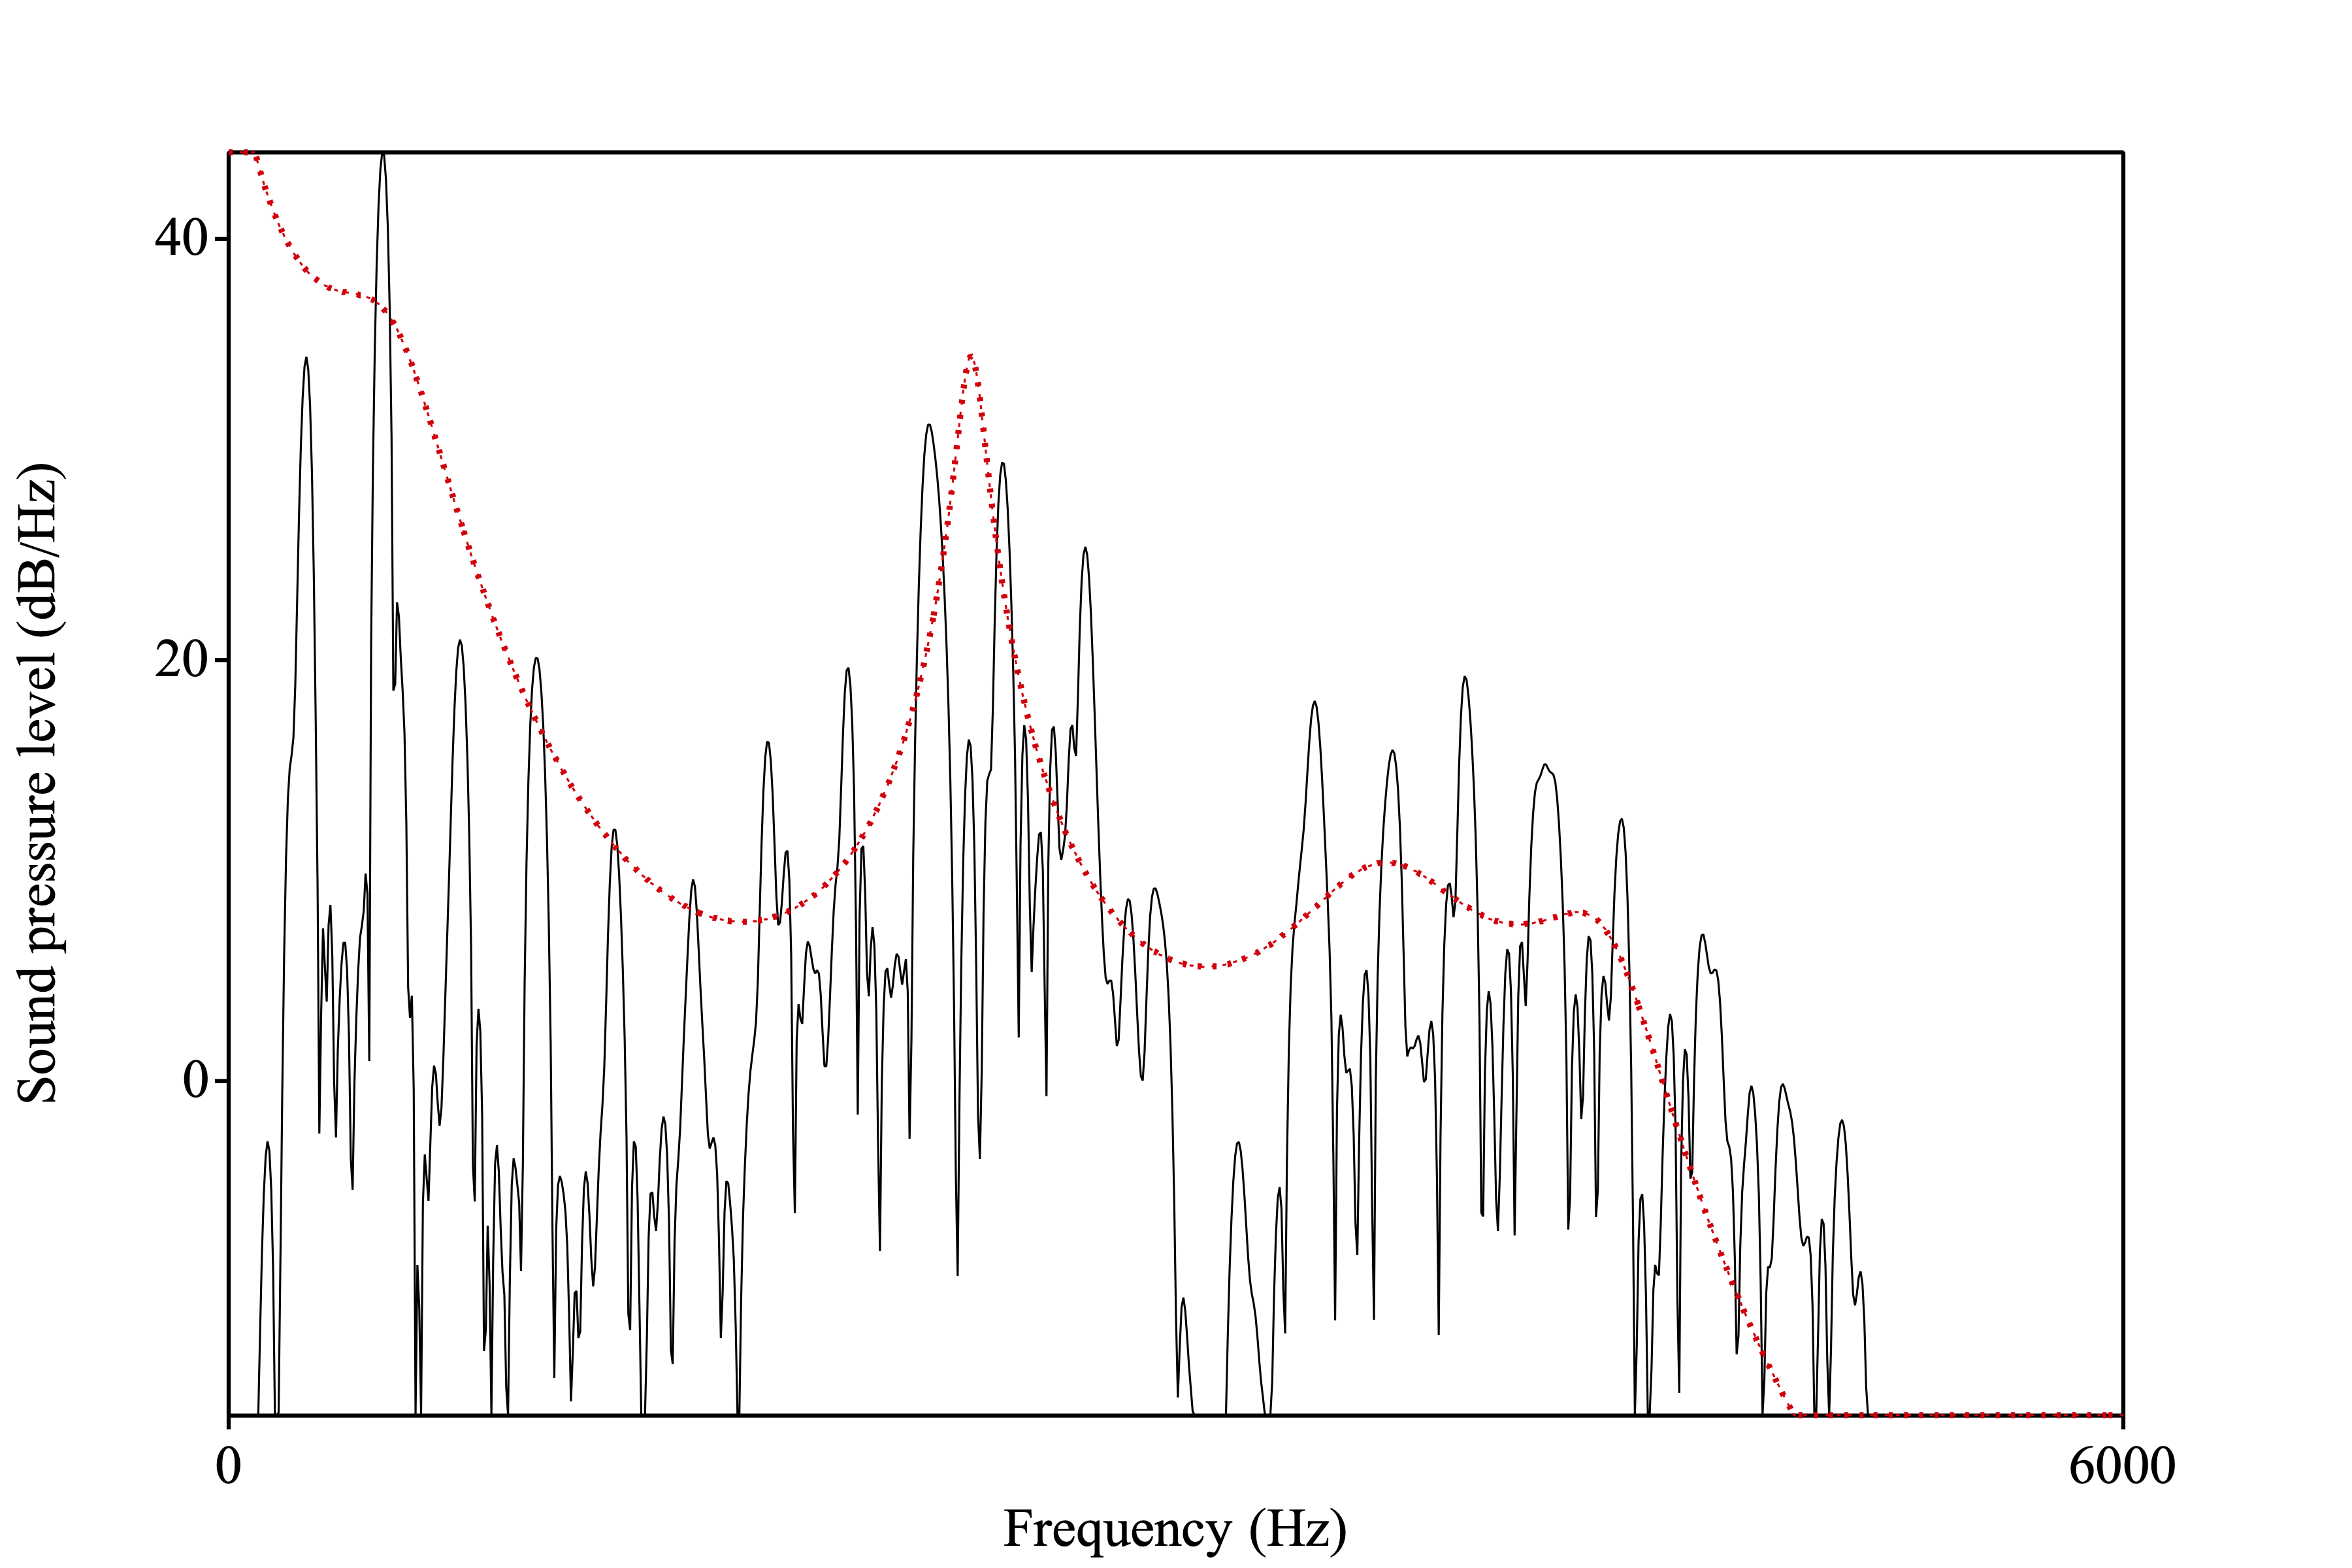
\includegraphics[width=0.9\textwidth]{../Harmonics.png}
	\caption{Spectral slice with LPC smoothed line overlaid for the vowel [e]. The harmonics in the spectral slice are represented by each of the dark peaks. The leftmost black solid line peak is the first harmonic (H1) and each subsequent peak represents the next highest harmonic (H2 through H\textit{n}). The red dotted line represents an LPC smoothed line which identifies the formants by the peaks. Each of the harmonics that are closest to the formant peak is identified as A1 through A\textit{n}.}
	\label{fig:Harmonics}
\end{figure}

When conducting spectral-tilt measurements, there are two types of measurements that can be made: corrected and uncorrected. The status of corrected or uncorrected refers to whether or not the influence of formants are taken into account (\cite{garellekPhoneticsVoice2019} provides a good overview of the differences). Most previous studies have not used corrected measure but have been focused on a single vowel /a/ because it minimizes the effects of the first formant \citep{espositoVariationContrastivePhonation2010}. Corrected measures take the formants into account during calculation and minimizes their influences. Fortunately, most software that is used for calculating the acoustic measurements such as VoiceSauce \citep{shueVOICESAUCEProgramVoice2009} and PraatSauce \citep{kirbyPraatSauce2022} produces both corrected and uncorrected values. 

A second type of spectral measure that one often encounters are harmonic-to-noise ratios. Harmonic-to-noise ratios refer to the difference in amplitude between the harmonic and inharmonic components of the source spectrum, as measured in the cepstral domain \citep{dekromCepstrumBasedTechniqueDetermining1993}. Frequently these harmonics-to-noise ratios take the form of a Cepstral Peak Prominence (CPP) measurement \citep{hillenbrandAcousticCorrelatesBreathy1994}.

In determining whether or not a given measure corresponds to a given phonation several patterns have been described and validated by many authors. A summary of these findings are given in \citet{garellekPhoneticsVoice2019} where it is noted that when the values of the spectral-tilt measurement are higher than that of the modal's spectral-tilt measurement and the CPP value is lower than the modal's CPP value this more than likely indicates a vowel with breathy phonation. If, however, the spectral-tilt measurements are lower than the modal's spectral-tilt measurements and the CPP value is lower than the modal's CPP value this more than likely indicates a vowel with creaky phonation. This means that if the acoustic measurements for the SLZ phonation types match these findings we can be fairly confident that we are dealing with breathy and creaky phonation. 

The rest of this section will describe the methods, results, and discussion of an acoustic analysis into SLZ's phonation. 

%------------------------------------
\subsection{Methods} \label{sec:Methods}
%------------------------------------

Due to the impact of the COVID-19 pandemic, only two native language speakers of SLZ were able to take part in this study (one male; one female). Both speakers live in Santa Cruz, CA and data collection was done remotely using Zencastr\footnote{\href{https://zencastr.com/}{https://zencastr.com/}}, a professional podcasting website, (44.1kHz, 16-bit) or in-person outside in a well ventilated location, using a Zoom H4n handheld recorder (44.1kHz, 16-bit). Participates were recorded saying approximately 100 words in the carrier sentence \textit{shnia' X chone las} `I say X three times'. This phrase was repeated three times. 

After the elicitations were completed the audio was uploaded into ELAN \citep{wittenburgELANProfessionalFramework2006} for initial segmentation into sentences. This was then followed by segmenting of the vowel portion in Praat \citep{boersmaPraatDoingPhonetics2021}. These segments were then inputted to VoiceSauce \citep{shueVOICESAUCEProgramVoice2009} were each vowel was resampled at 16kHZ for acoustic measurement. The acoustic measurements of VoiceSauce were then analyzed in R \citep{rcoreteamLanguageEnvironmentStatistical2021}. In order to investigate the differences in timing, each vowel was normalized for time and following \citet{garellekAcousticConsequencesPhonation2011}, the resulting measurements were averaged for each third of the vowel. 

%------------------------------------
\subsection{Spectral-tilt results} \label{sec:Results}
%------------------------------------

In plotting the spectral-tilt measurements, we find that the results follow some of the established patterns and deviates in others. This section will first discuss the results of the H1-H2 measurements for the both FSR and RD, the H1-A3 measurements for FSR and RD, and the CPP measurements for FSR and RD. 

%------------------------------------
\subsubsection{H1-H2 results} \label{sec:H1H2}
%------------------------------------

The clearest result that was able to be gleaned from the H1-H2 measurements show that the breathy voice is much lower than the measurement for modal vowels throughout much of the vowel. This can be seen in Figures~\ref{fig:FSRh1h2first}, \ref{fig:h1h2second}, and \ref{fig:h1h2third}.

\begin{figure}[!ht]
	\centering
	\begin{subfigure}{.5\textwidth}
		\centering
		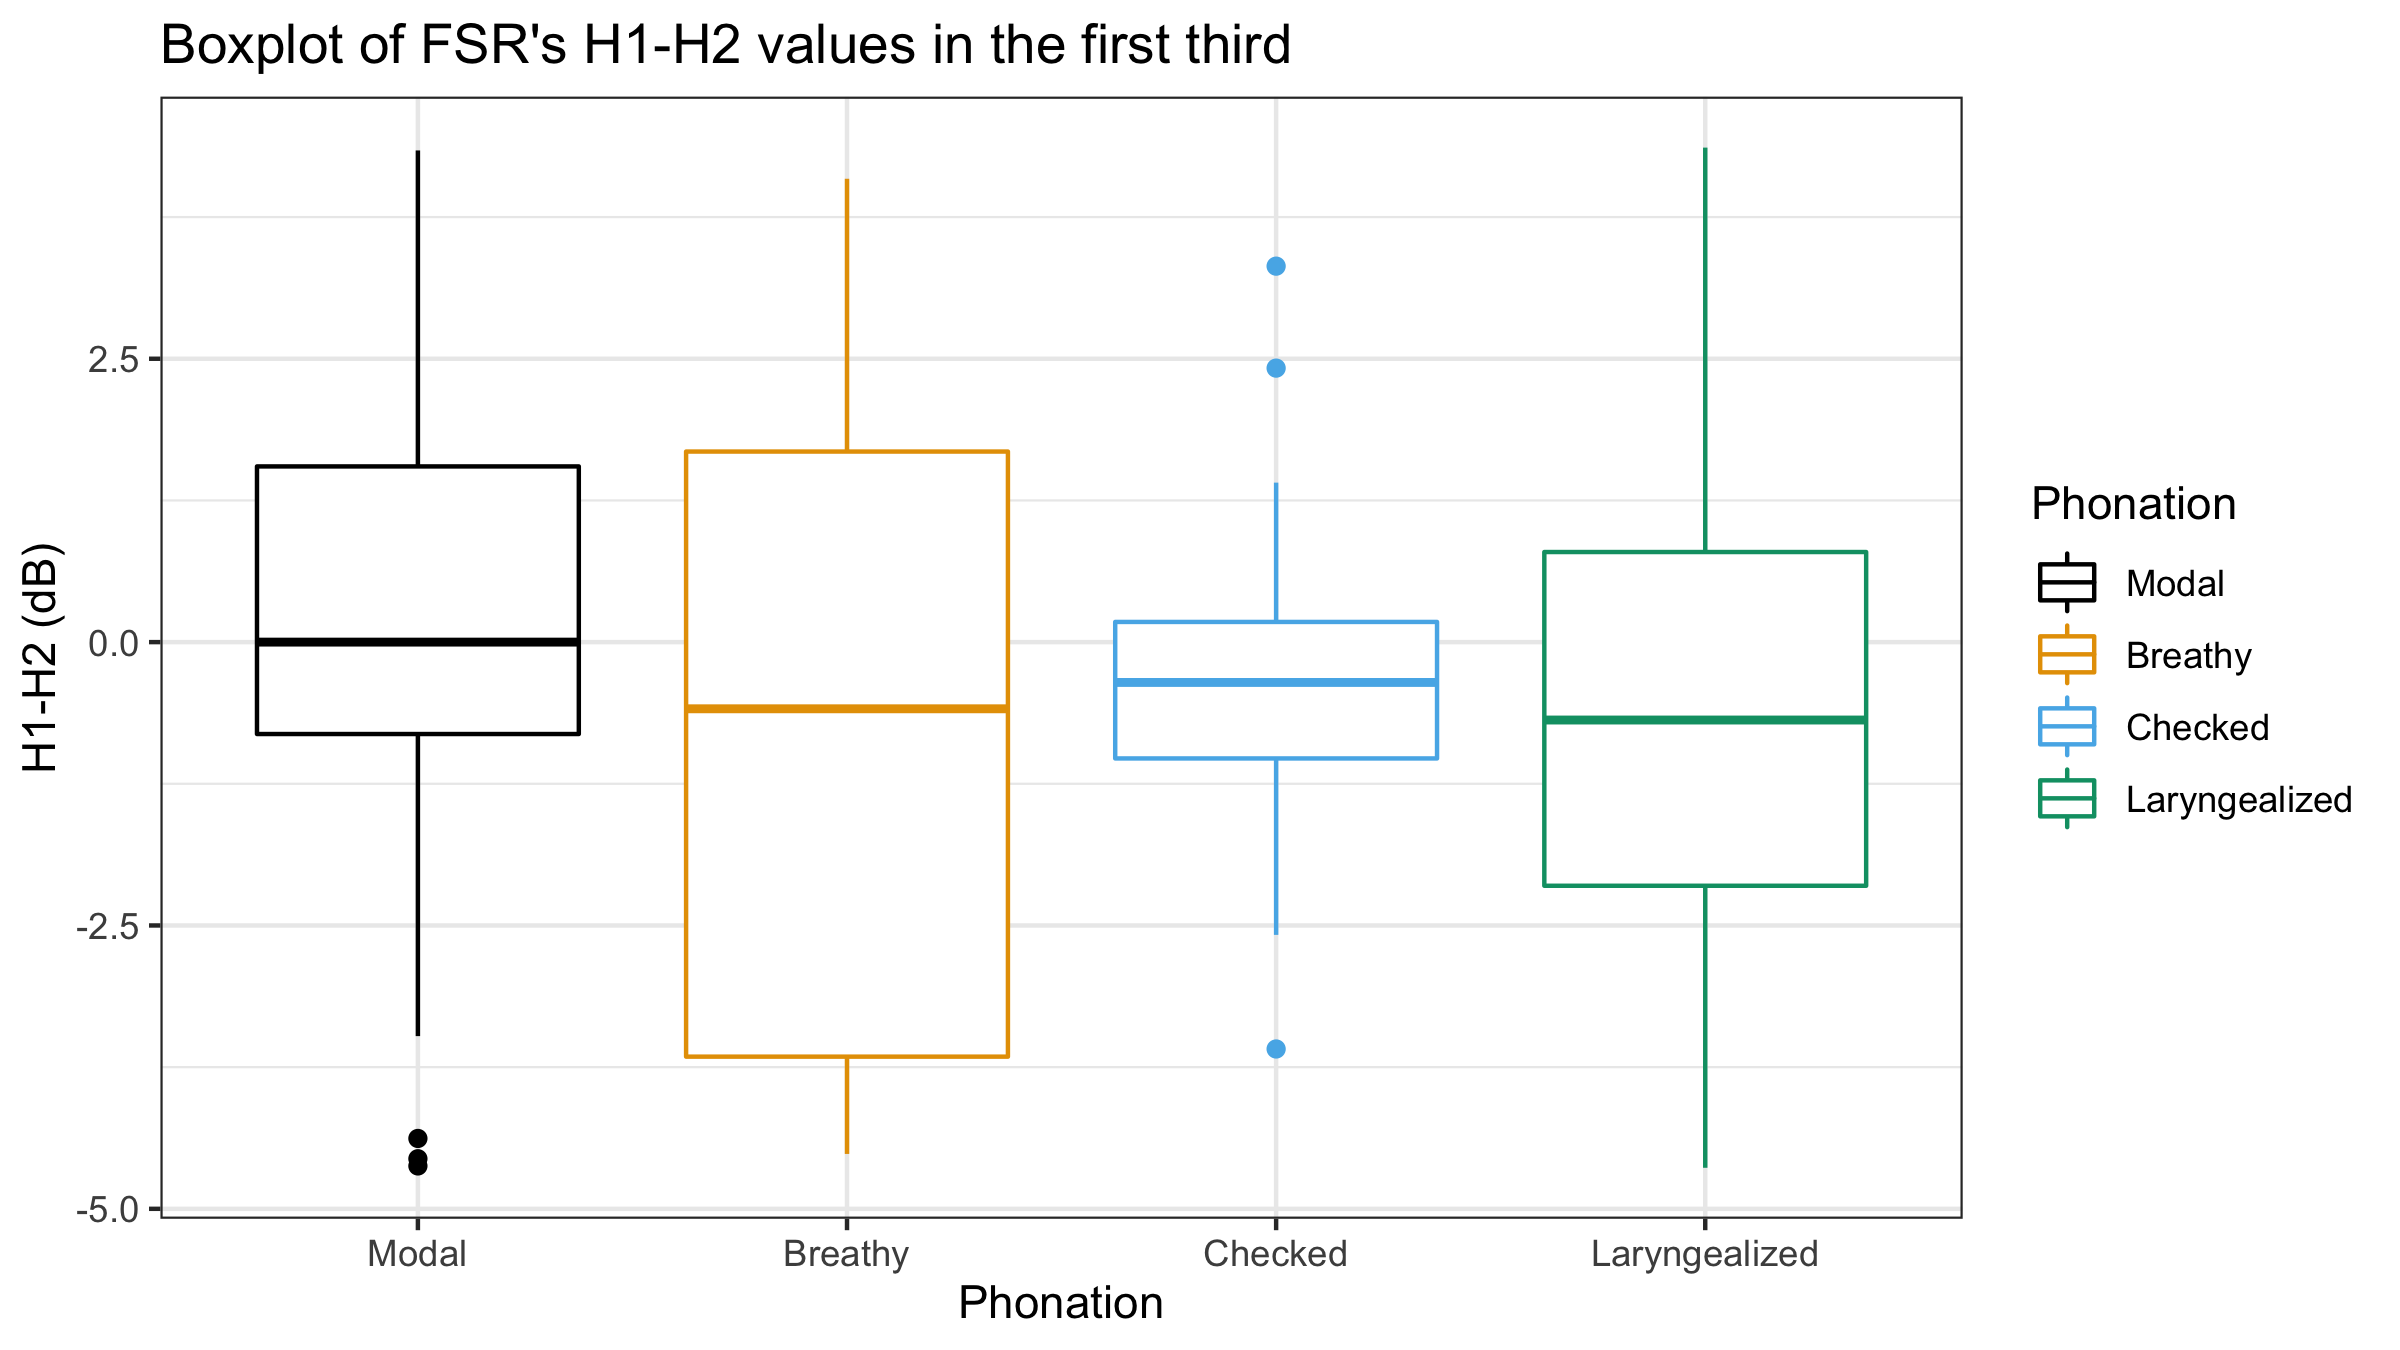
\includegraphics[width=0.9\textwidth]{../mean_FSR_h1h2_1st.png}
		\caption{FSR's H1-H2 values.}
		\label{fig:FSRh1h2first} 
	\end{subfigure}%
	\begin{subfigure}{.5\textwidth}
		\centering
		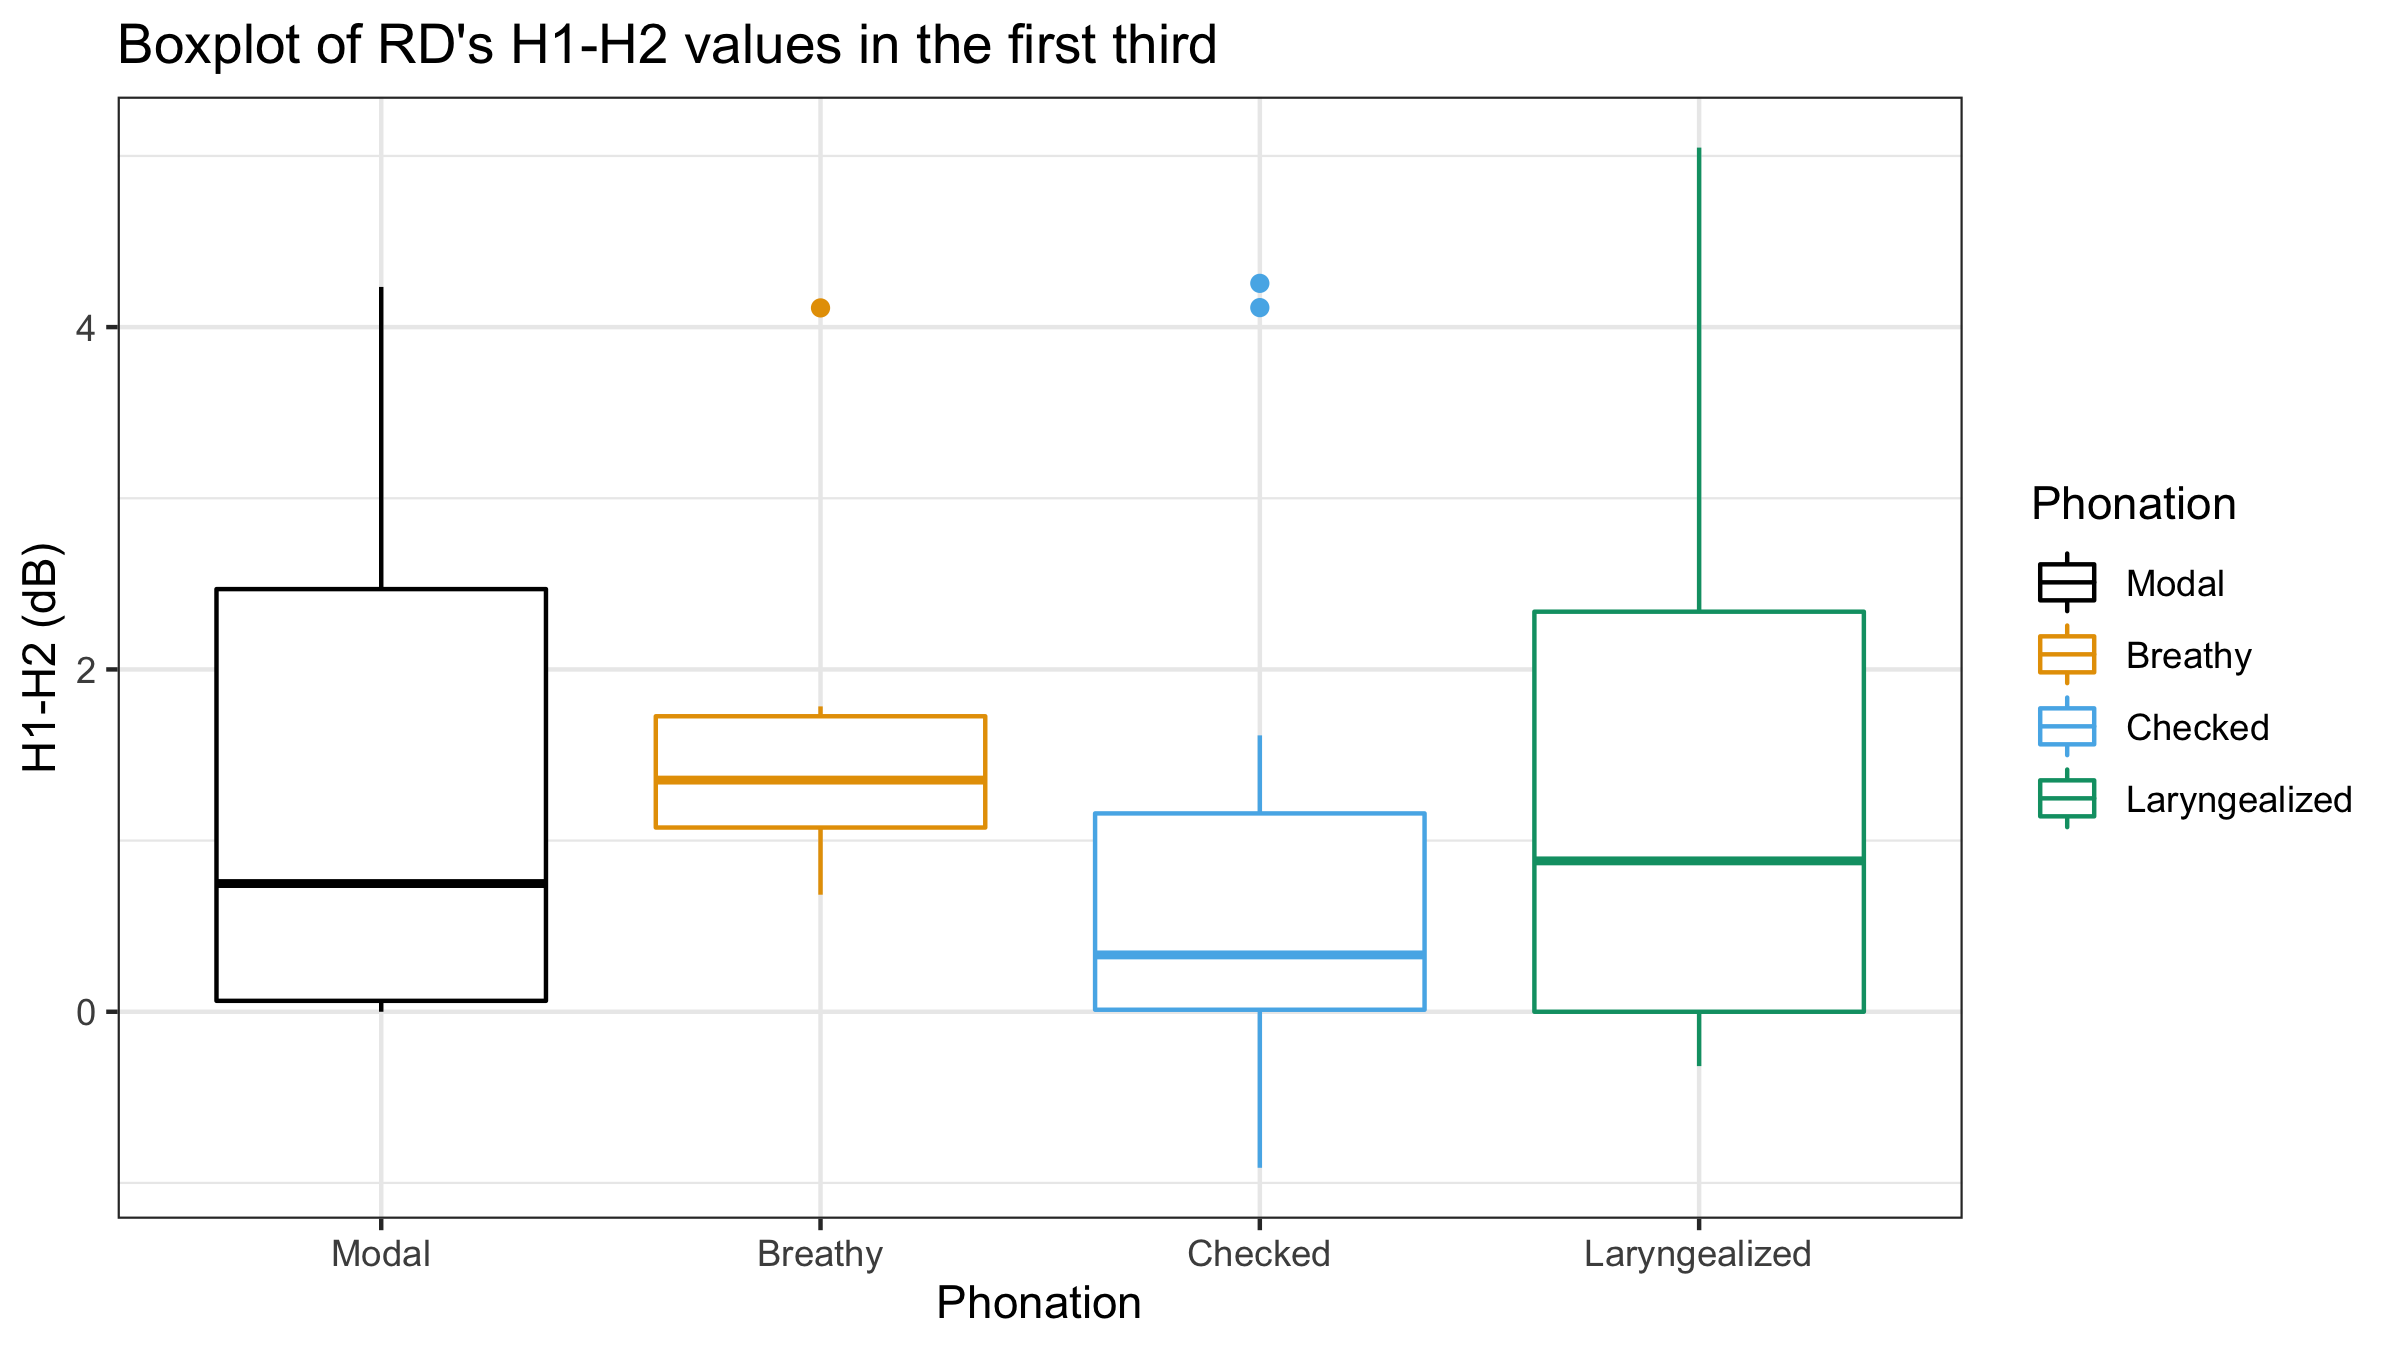
\includegraphics[width=0.9\textwidth]{../mean_RD_h1h2_1st.png}
		\caption{RD's H1-H2 values.}
		\label{fig:RDh1h2first} 
	\end{subfigure}
	\caption{Mean H1-H2 values for the first third of the vowel according to each phonation type. }
	\label{fig:h1h2first}
\end{figure}

Additionally, in the first third of the vowel as shown in Figure~\ref{fig:h1h2first}, we see that the mean values for checked vowels are lower than those for modal vowels. This is true for both FSR and RD. In regards to laryngealized vowels the mean value for H1-H2 is nearly identical to that for modal vowels for RD. However, for FSR the value is lower.

\begin{figure}[!ht]
	\centering
	\begin{subfigure}{.5\textwidth}
		\centering
		\includegraphics[width=0.9\textwidth]{../mean_FSR_h1h2_2nd.png}
		\caption{FSR's H1-H2 values.}
		\label{fig:FSRh1h2second} 
	\end{subfigure}%
	\begin{subfigure}{.5\textwidth}
		\centering
		\includegraphics[width=0.9\textwidth]{../mean_RD_h1h2_2nd.png}
		\caption{RD's H1-H2 values.}
		\label{fig:RDh1h2second} 
	\end{subfigure}
	\caption{Mean H1-H2 values for the second third of the vowel according to each phonation type.}
	\label{fig:h1h2second}
\end{figure}

In looking at the second third of each vowel, we observe very similar results as that for the first third except that there is a more pronounced decline in values for breathy vowels with them being much lower than modal vowels, see Figure~\ref{fig:h1h2second}. The results for checked and laryngealized vowels are still nearly identical to those in Figure~\ref{fig:h1h2first}.

\begin{figure}[!ht]
	\centering
	\begin{subfigure}{.5\textwidth}
		\centering
		\includegraphics[width=0.9\textwidth]{../mean_FSR_h1h2_3rd.png}
		\caption{FSR's H1-H2 values.}
		\label{fig:FSRh1h2third} 
	\end{subfigure}%
	\begin{subfigure}{.5\textwidth}
		\centering
		\includegraphics[width=0.9\textwidth]{../mean_RD_h1h2_3rd.png}
		\caption{RD's H1-H2 values.}
		\label{fig:RDh1h2third} 
	\end{subfigure}
	\caption{Mean H1-H2 values for the final third of the vowel according to each phonation type. }
	\label{fig:h1h2third}
\end{figure}

In the final third of the vowel, we continue to see breathy vowels having a lower H1-H2 value than modal vowels, which runs against our expectations for breathy vowels. Breathy vowels should have a higher value for H1-H2 than modal vowels. In FSR's values for checked and laryngealized vowels, the values are still roughly the same as they were for previous portions of the vowel. RD, however, shows H1-H2 values for checked and laryngealized vowels that are lower than the values for the modal vowel. 

%------------------------------------
\subsubsection{H1-A3 results} \label{sec:H1A3}
%------------------------------------

In turning to the H1-A3 spectral-tilt measurement that \citet{espositoVariationContrastivePhonation2010} found useful for Central Valley Zapotec, several observations quickly become apparent. The most striking is the higher H1-A3 value found for breathy vowels in all portions of the vowel. This observation is true for both FSR and RD. 

\begin{figure}[!h]
	\centering
	\begin{subfigure}{.5\textwidth}
		\centering
		\includegraphics[width=0.9\textwidth]{../mean_FSR_h1a3_First.png}
		\caption{FSR's H1-A3 values.}
		\label{fig:FSRh1a3first} 
	\end{subfigure}%
	\begin{subfigure}{.5\textwidth}
		\centering
		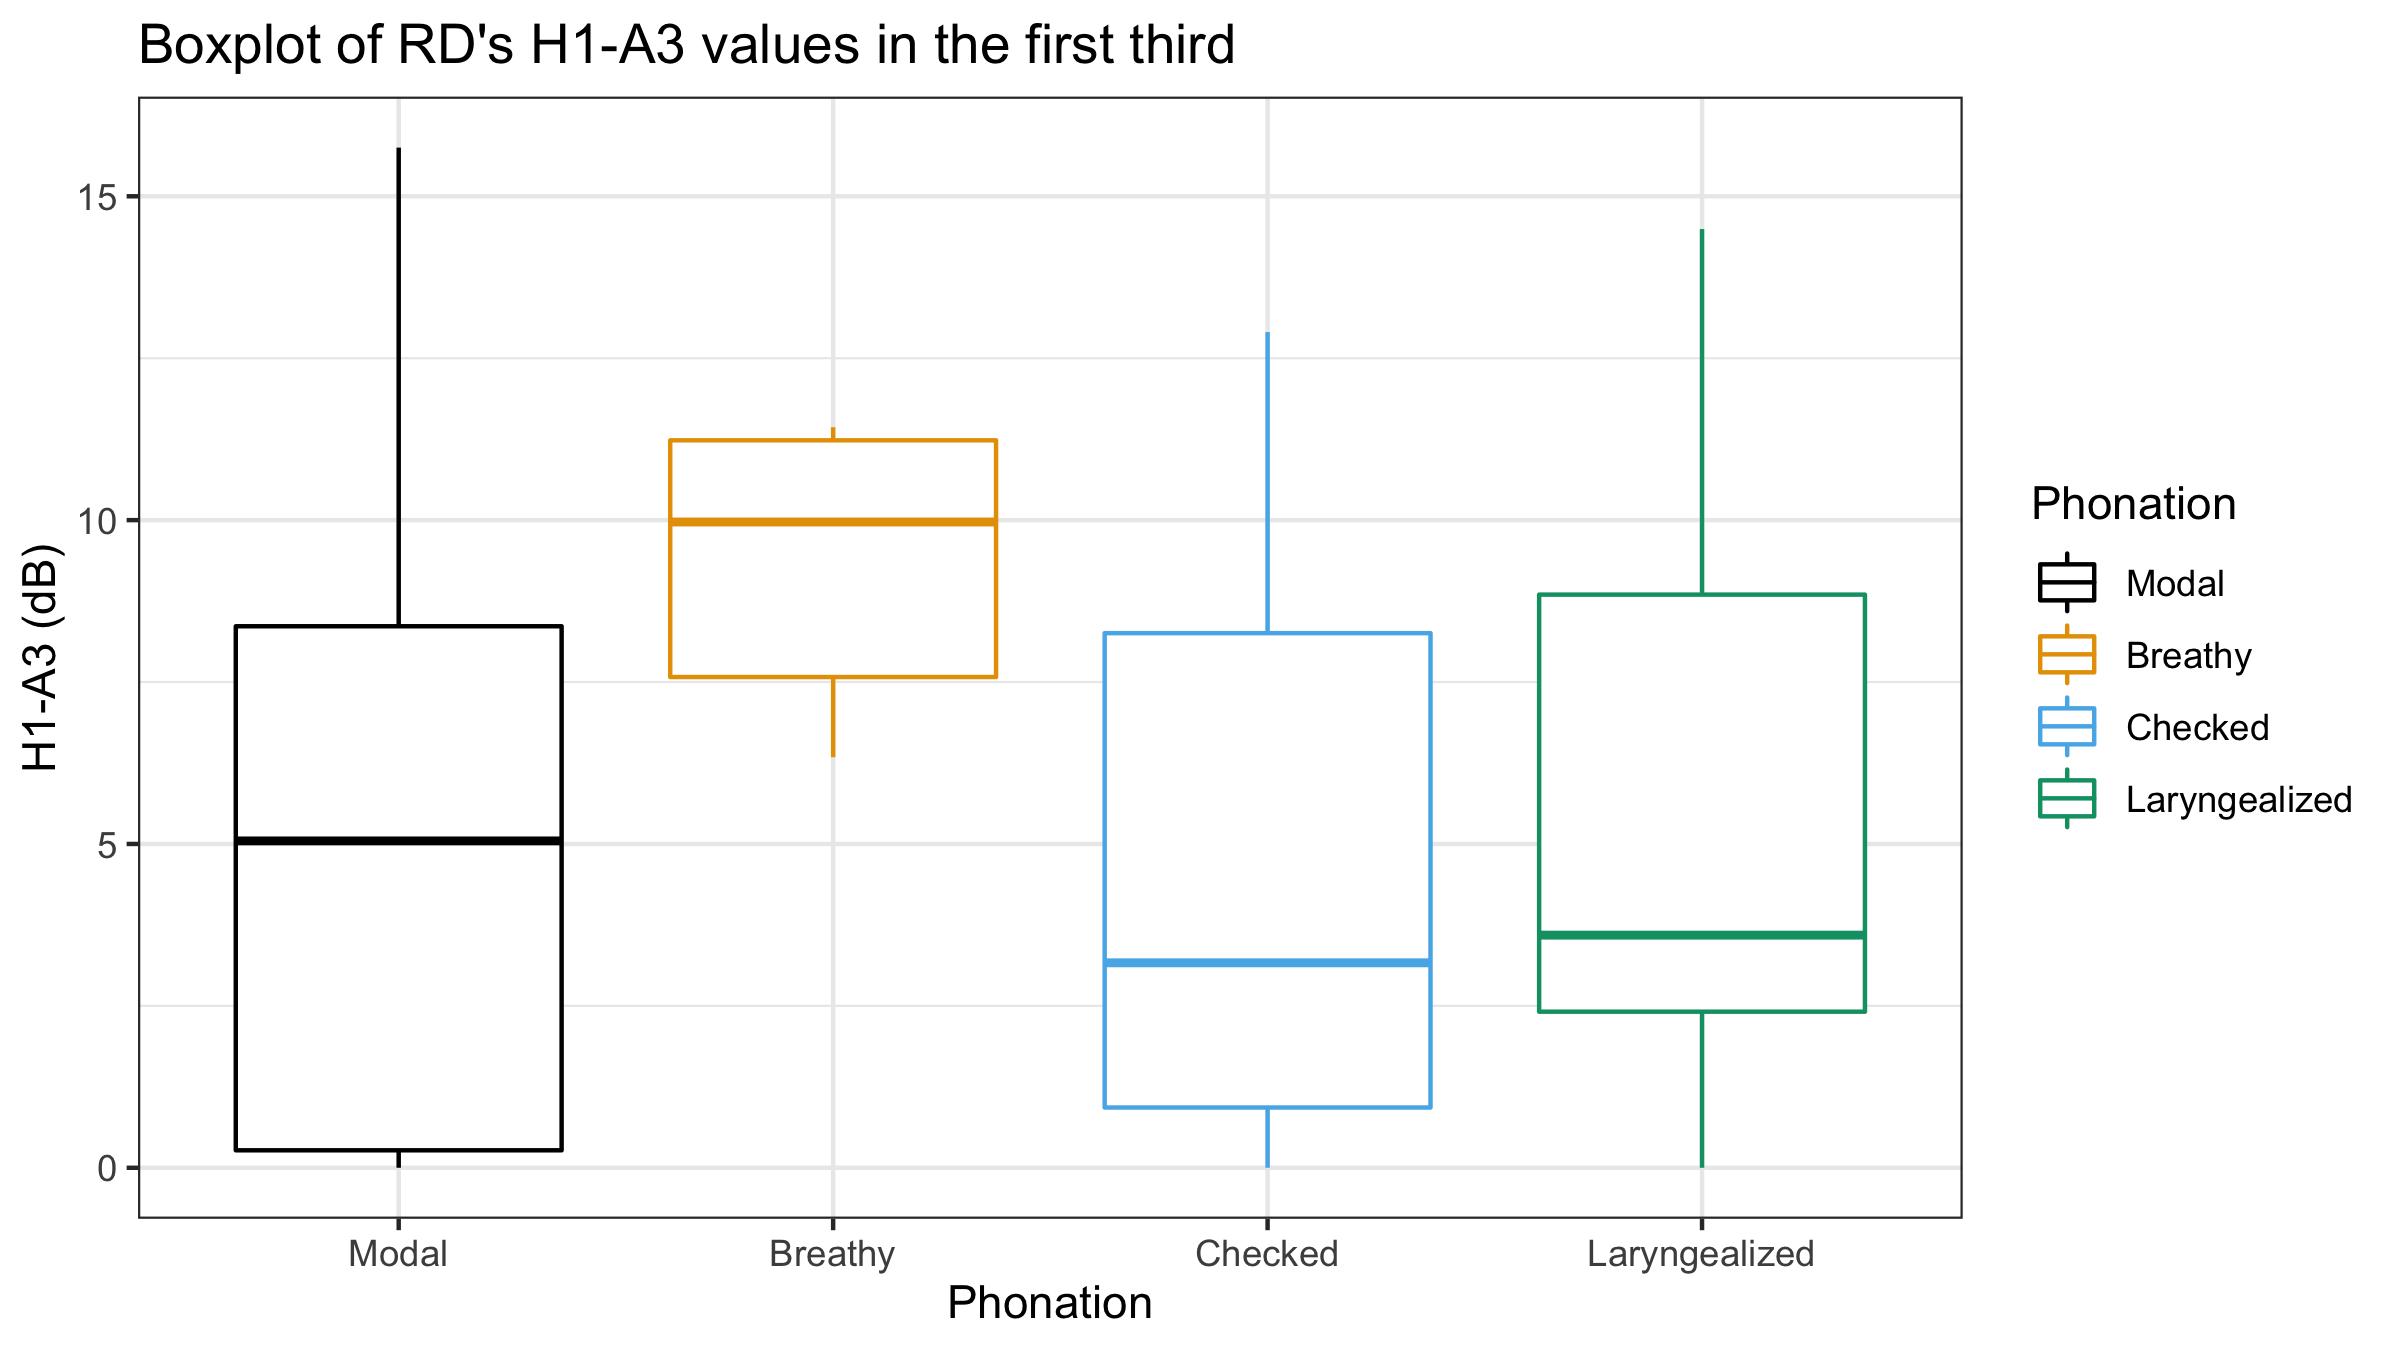
\includegraphics[width=0.9\textwidth]{../mean_RD_h1a3_First.png}
		\caption{RD's H1-A3 values.}
		\label{fig:RDh1a3first} 
	\end{subfigure}
	\caption{H1-A3 values for FSR (a) and RD (b) for the first third of the vowel. }
	\label{fig:h1a3first}
\end{figure}

In the first third of the vowel, RD's mean value for H1-A3 is lower than the modal's H1-A3 value. However, there is a large degree of overlap between modals, checked, and laryngealized H1-A3 values, as evidenced by the boxes covering the same regions, see Figure~\ref{fig:h1a3first}. 

\begin{figure}[!h]
	\centering
	\begin{subfigure}{.5\textwidth}
		\centering
		\includegraphics[width=0.9\textwidth]{../mean_FSR_h1a3_Second.png}
		\caption{FSR's H1-A3 values.}
		\label{fig:FSRh1a3second} 
	\end{subfigure}%
	\begin{subfigure}{.5\textwidth}
		\centering
		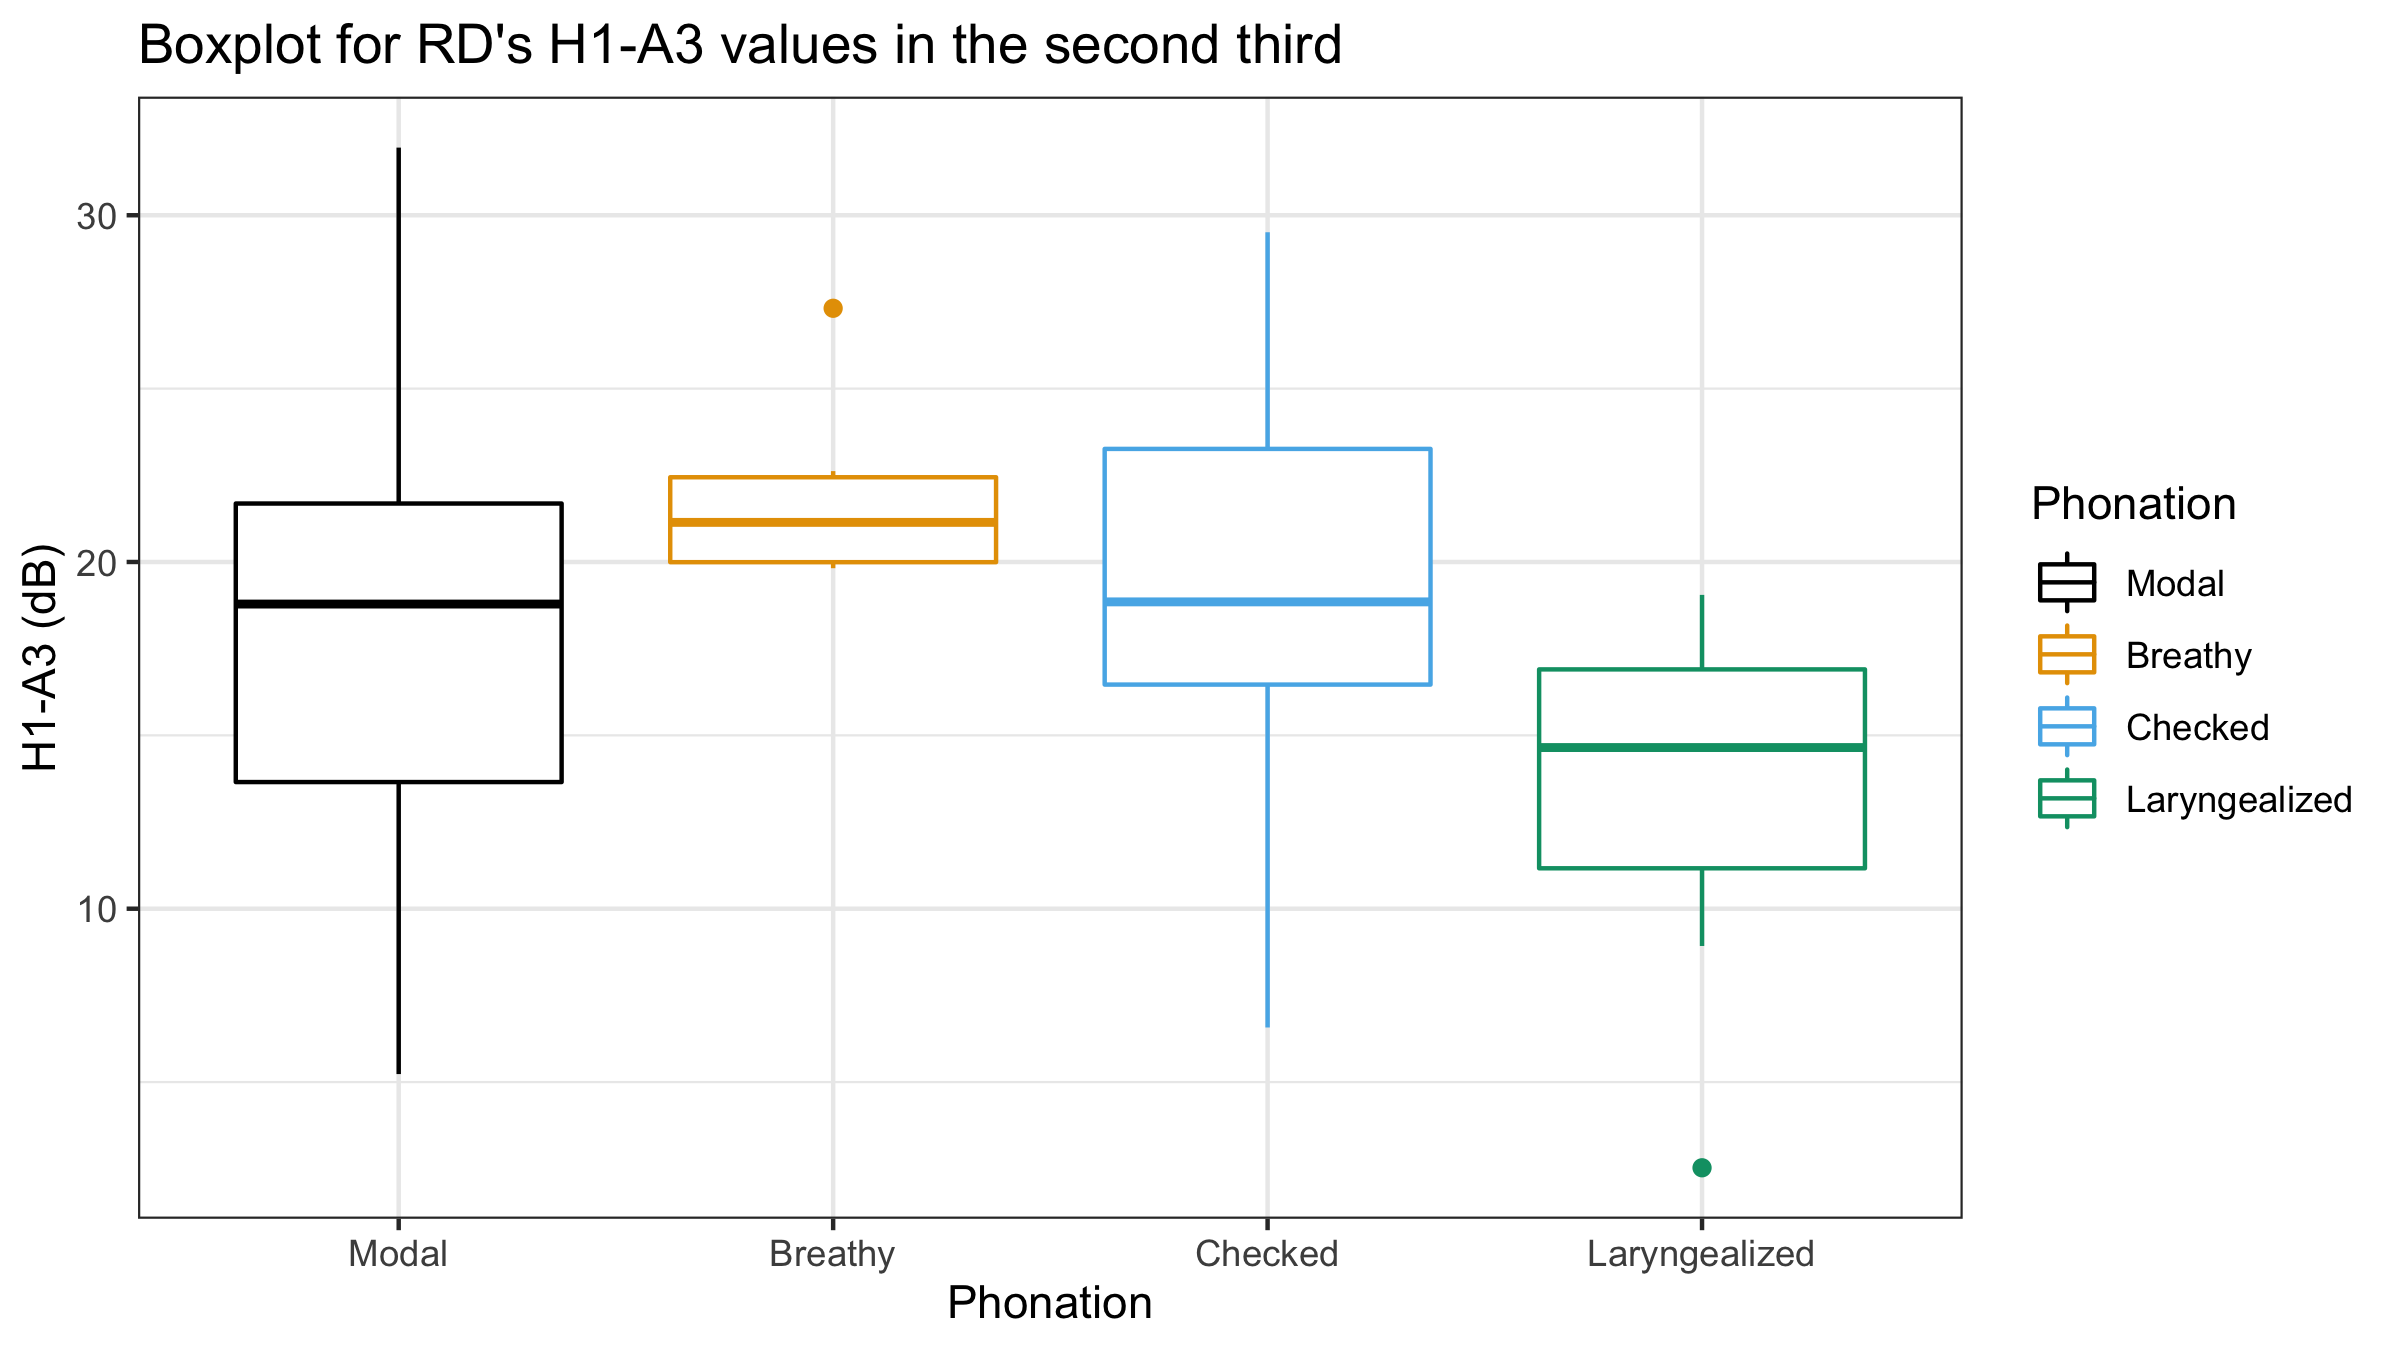
\includegraphics[width=0.9\textwidth]{../mean_RD_h1a3_Second.png}
		\caption{RD's H1-A3' values.}
		\label{fig:RDh1a3second} 
	\end{subfigure}
	\caption{H1-A3 values for FSR (a) and RD (b) for the second third of the vowel. }
	\label{fig:h1a3second}
\end{figure}

In the second third of the vowel, Figure~\ref{fig:h1a3second}, the breathy vowel continues to be higher than the modal vowel. The checked and laryngealized vowels H1-A3 values for FSR are uninformative because of the large degree of overlap. For RD, these same measurements show a lower H1-A3 value than the modals which is consistent with creakier productions of vowels. This lower H1-A3 continues throughout the rest of the vowel for laryngealized vowels, see Figure~\ref{fig:RDh1a3third}. This behavior is consistent with the observation that RD performs creaky voice throughout their production of laryngealized vowels. For the checked vowels, the measurements are very similar to those of the modal vowel. 

In looking at the final portion of the vowels, Figure~\ref{fig:h1a3third}, the measurements continue to show similar behavior to the second portion for both FSR and RD. However, one exception is the lower H1-A3 value for FSR's checked vowels, suggesting that FSR produces a period of creakiness in the last portion of the vowel.

\begin{figure}[!ht]
	\centering
	\begin{subfigure}{.5\textwidth}
		\centering
		\includegraphics[width=0.9\textwidth]{../mean_FSR_h1a3_third.png}
		\caption{FSR's H1-A3 values.}
		\label{fig:FSRh1a3third} 
	\end{subfigure}%
	\begin{subfigure}{.5\textwidth}
		\centering
		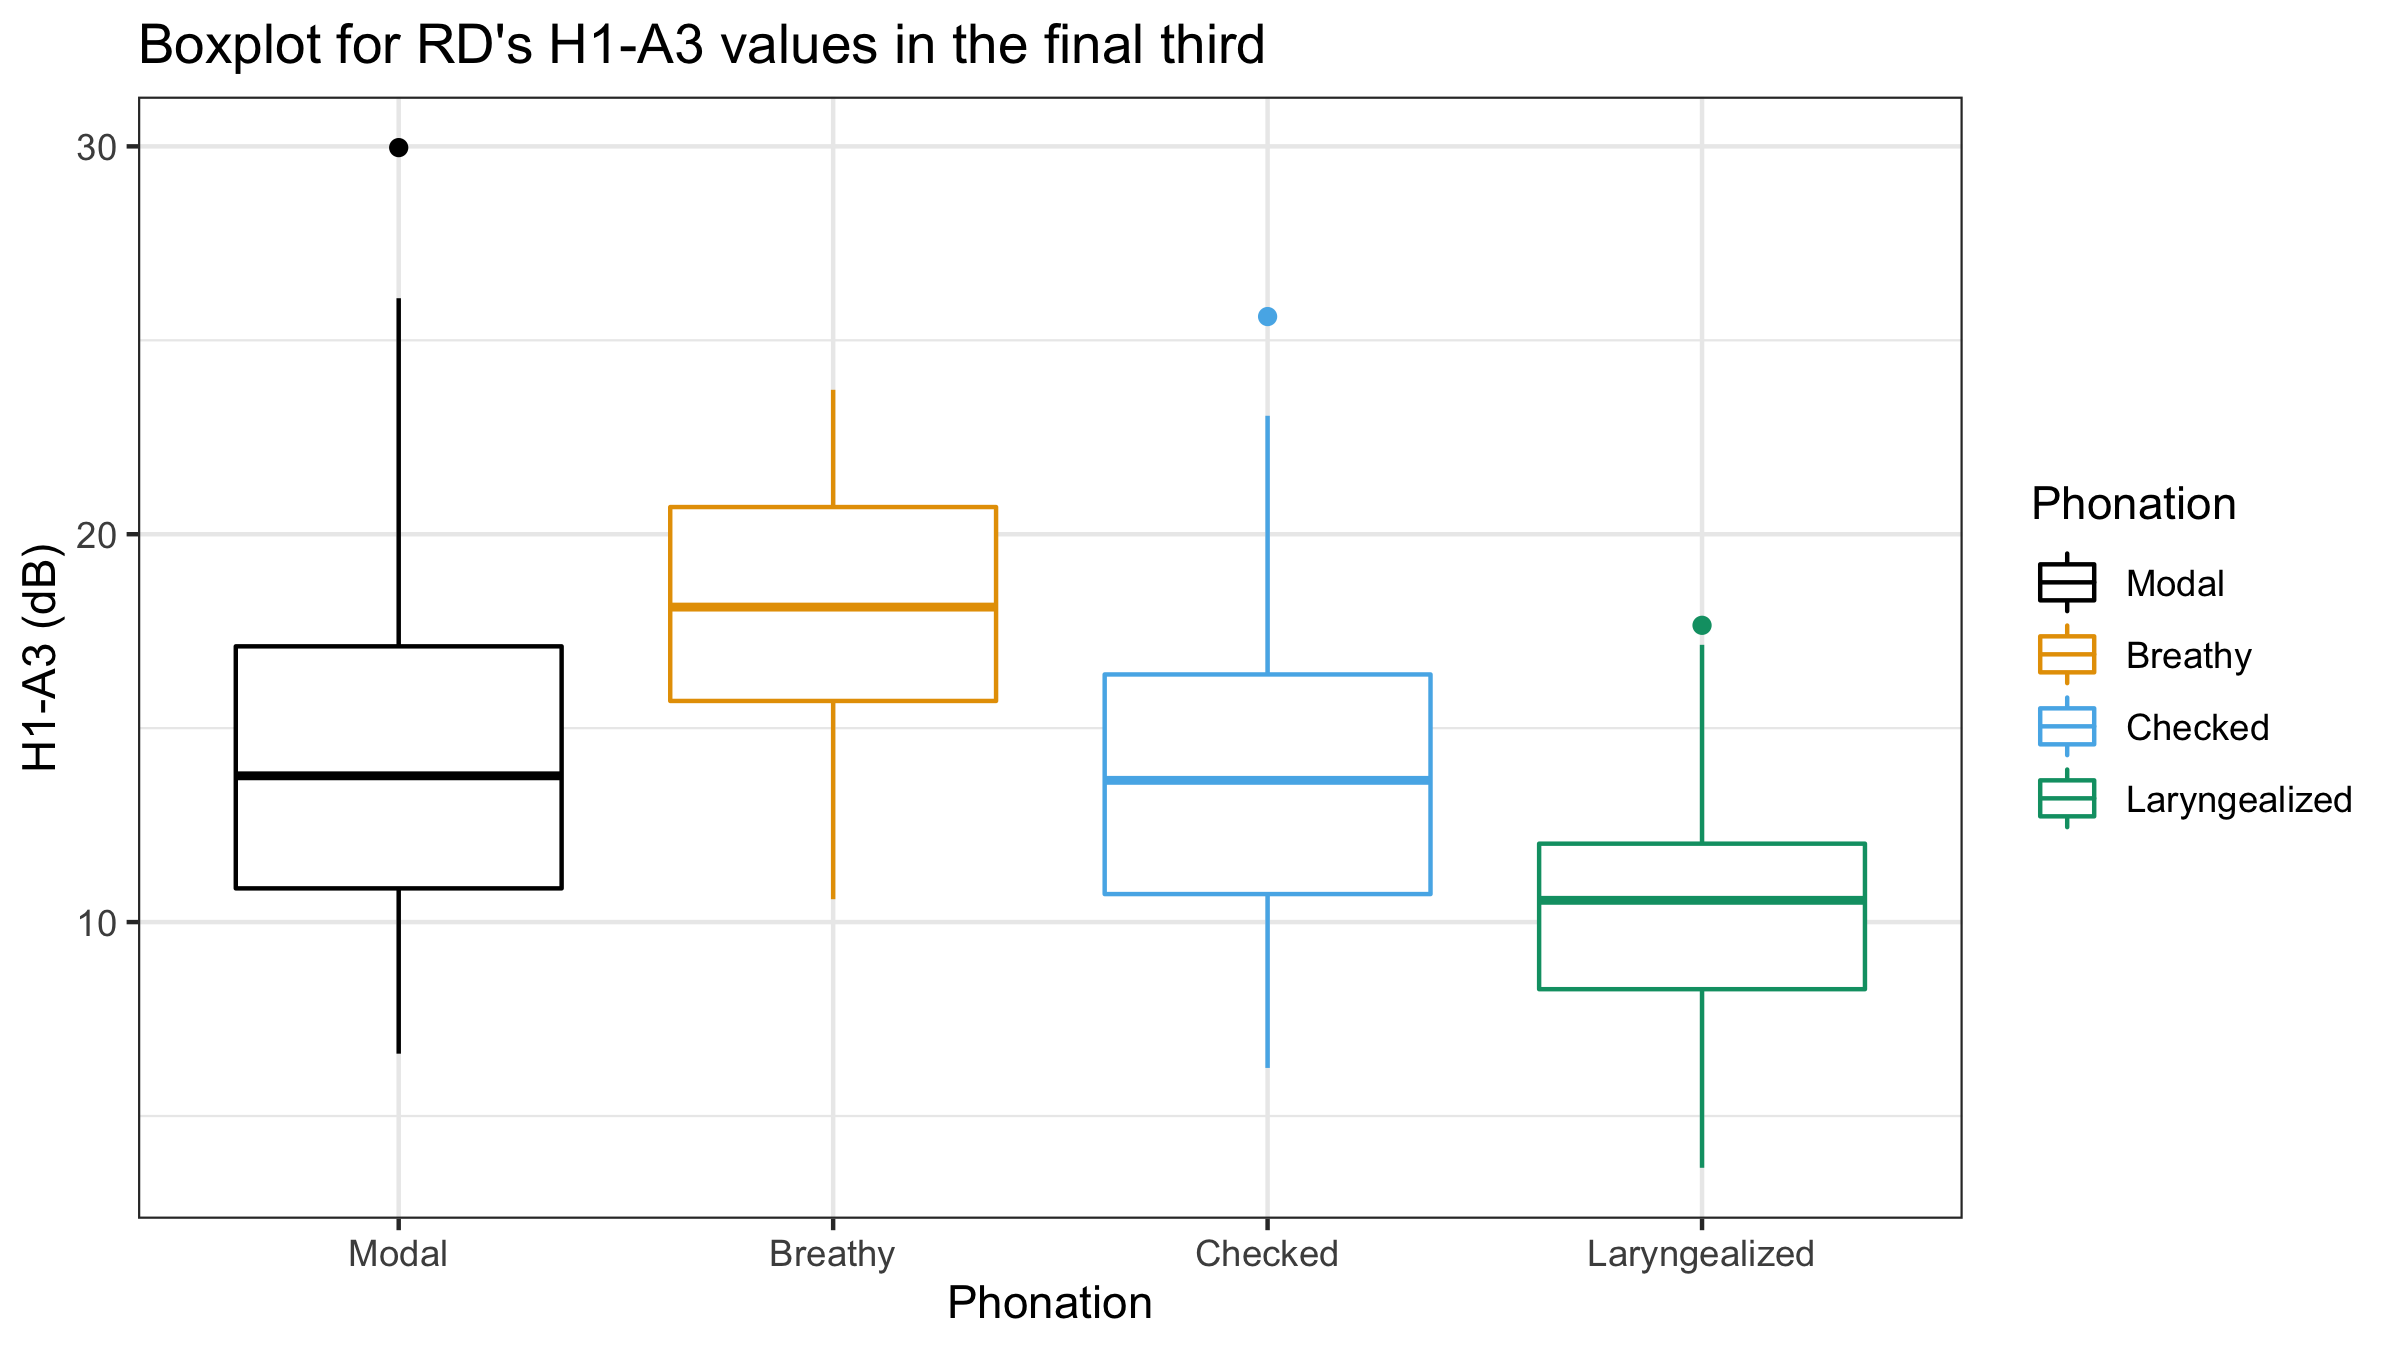
\includegraphics[width=0.9\textwidth]{../mean_RD_h1a3_third.png}
		\caption{RD's H1-A3 values.}
		\label{fig:RDh1a3third} 
	\end{subfigure}
	\caption{H1-A3 values for FSR (a) and RD (b) for the final third of the vowel. }
	\label{fig:h1a3third}
\end{figure}

%------------------------------------
\subsubsection{CPP results} \label{sec:CPP}
%------------------------------------

As previously mentioned at the start of Section~\ref{sec:Acoustics}, another measurement that is frequently encountered with spectral-tilt measurements is a Cepstral Peak Prominence (CPP) measurement \citep{hillenbrandAcousticCorrelatesBreathy1994}, which is a type of harmonics-to-noise ratio and indicates whether or not there is any aperiodicity in the signal. 

A CPP measurement for any vowel with non-modal phonation should be lower than the CPP measurement for modal vowels. When evaluating the CPP measurements for the same vowels and portions of a vowel, there are several observations that readily become apparent. The most noticeable observation is that for both speakers the breathy vowel's CPP value is consistently higher than the modal vowel's CPP value, which is opposite what is typically observed for non-modal phonation. When evaluating the checked vowel's CPP values, FSR had a lower value in the first third but the rest of the vowel shows values that are comparable to the modal vowel. For RD's checked vowels, the CPP shows that the mean is in fact lower than the modals in Figures~\ref{fig:RDcppfirst}, \ref{fig:RDcppsecond}, and \ref{fig:RDcppthird} but there is a large overlap in values. 

Laryngealized vowels show a different pattern. For FSR, the laryngealized vowel's CPP value is lower than the modal's CPP value in the second-third of the vowel only. For RD, however, the laryngealized vowels have the roughly the same values as the modal vowels throughout the thirds. 

\begin{figure}[!ht]
	\centering
	\begin{subfigure}{.5\textwidth}
		\centering
		\includegraphics[width=0.9\textwidth]{../mean_FSR_cpp_First.png}
		\caption{FSR's CPP values.}
		\label{fig:FSRcppfirst} 
	\end{subfigure}%
	\begin{subfigure}{.5\textwidth}
		\centering
		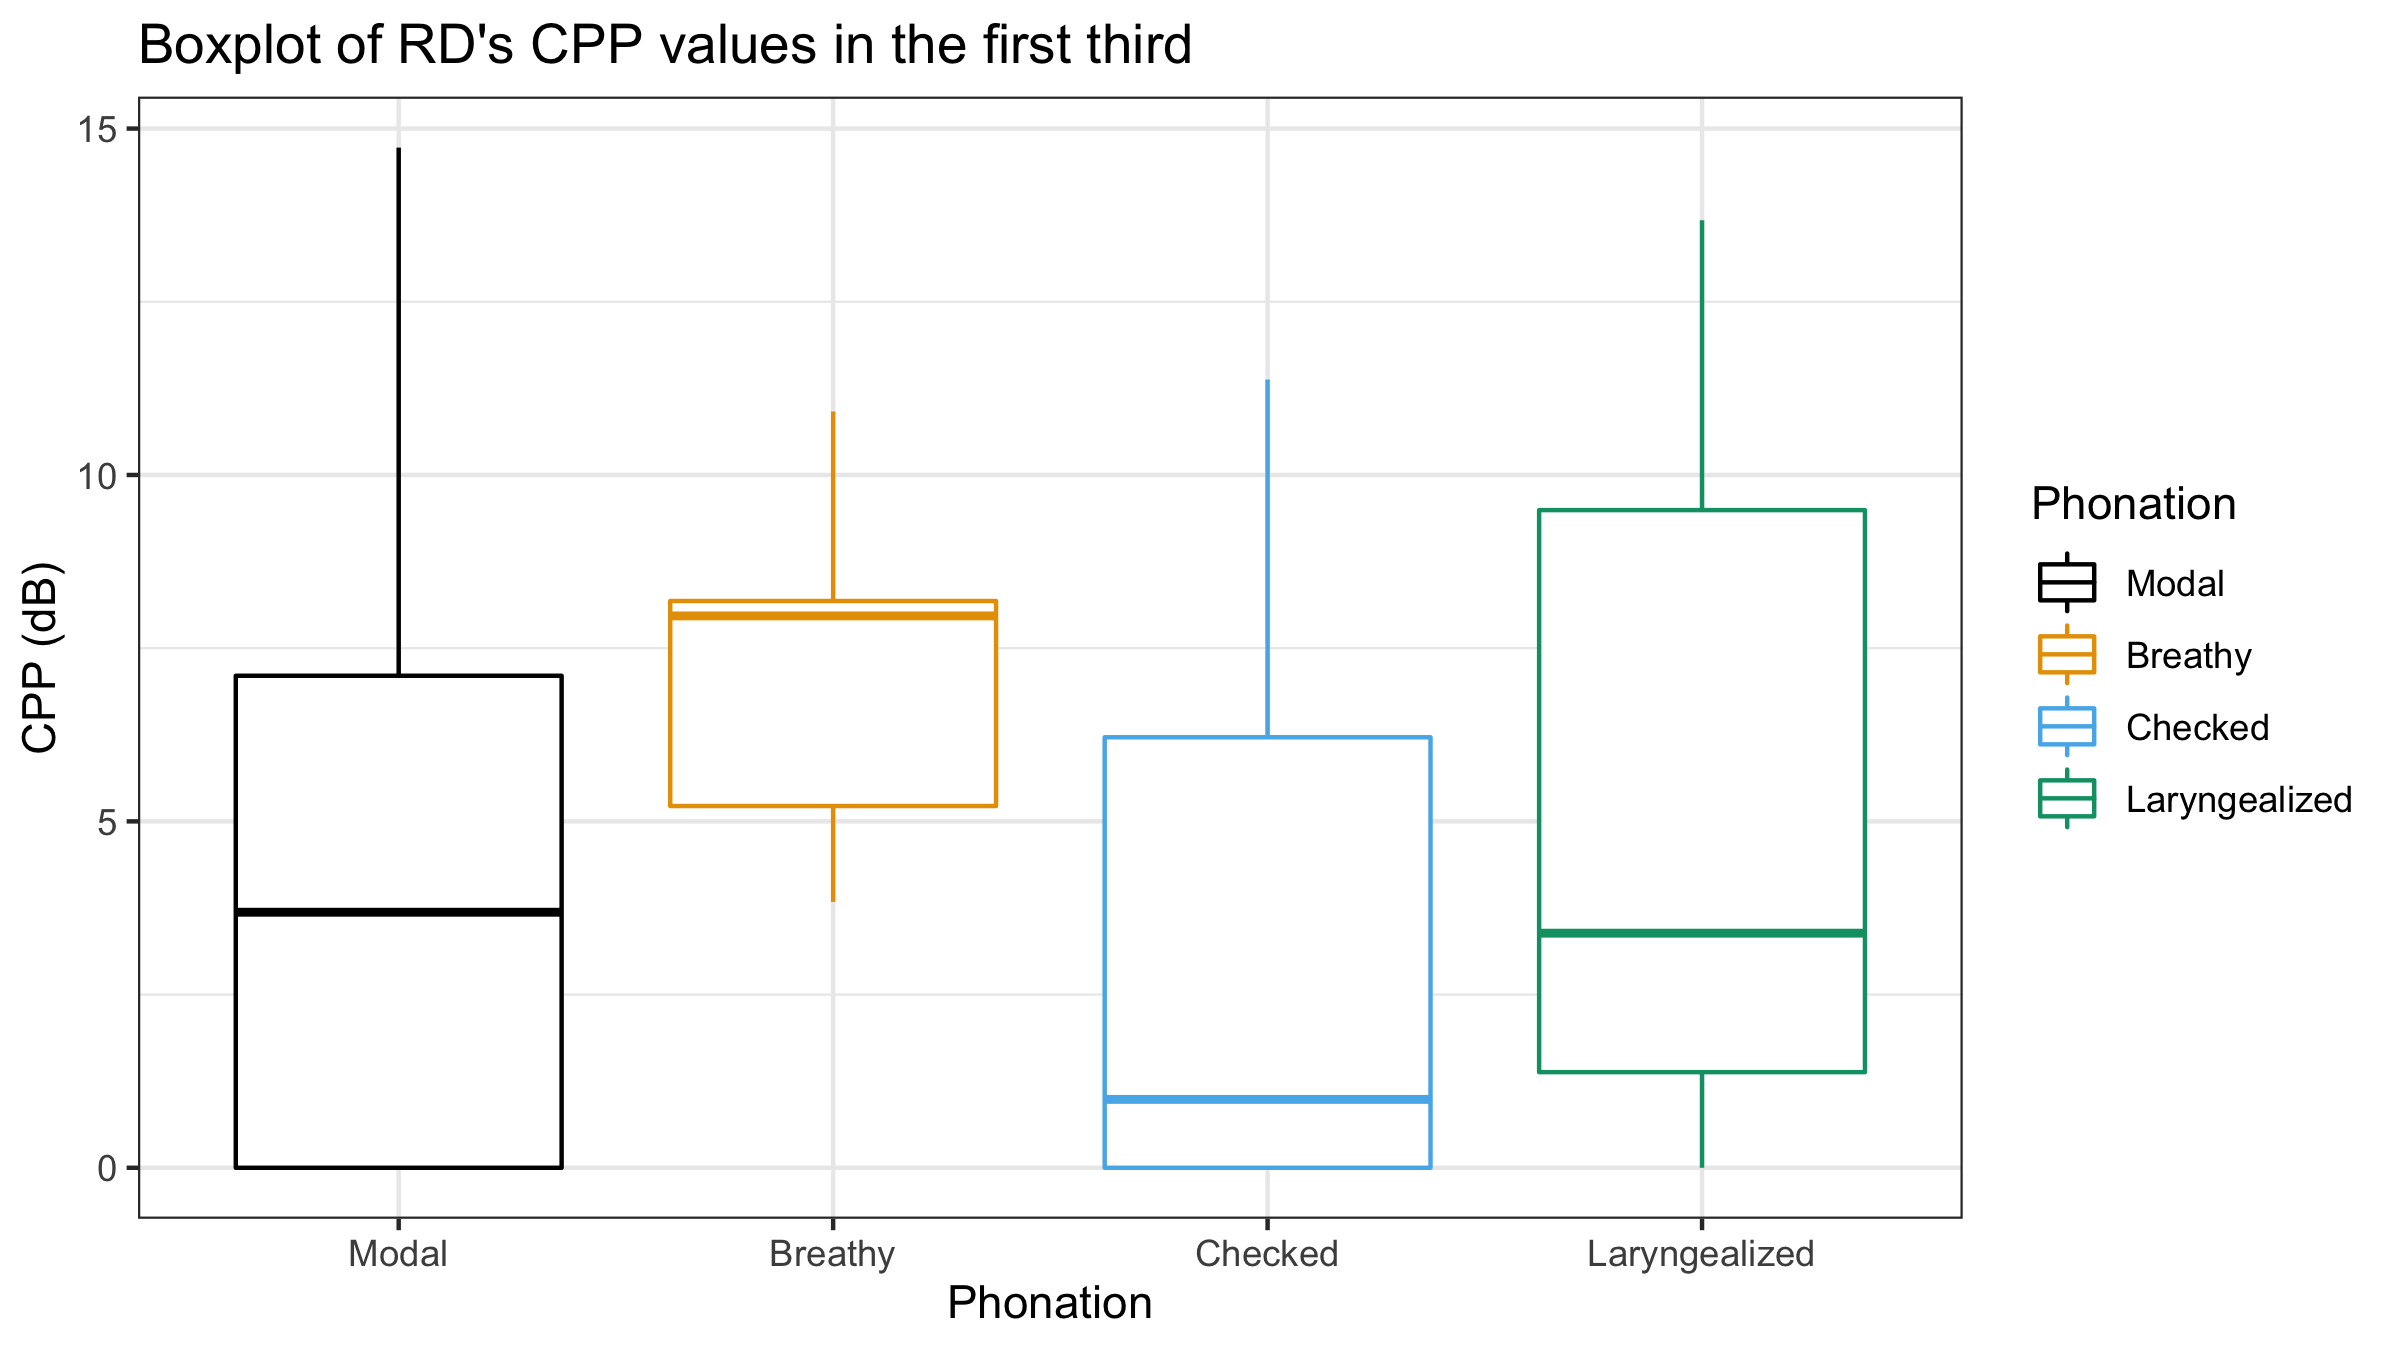
\includegraphics[width=0.9\textwidth]{../mean_RD_cpp_First.png}
		\caption{RD's CPP values.}
		\label{fig:RDcppfirst} 
	\end{subfigure}
	\caption{CPP values for FSR (a) and RD (b) for the first third of the vowel. }
	\label{fig:cppfirst}
\end{figure}

\begin{figure}[!ht]
	\centering
	\begin{subfigure}{.5\textwidth}
		\centering
		\includegraphics[width=0.9\textwidth]{../mean_FSR_cpp_Second.png}
		\caption{FSR's CPP values.}
		\label{fig:FSRcppsecond} 
	\end{subfigure}%
	\begin{subfigure}{.5\textwidth}
		\centering
		\includegraphics[width=0.9\textwidth]{../mean_RD_cpp_Second.png}
		\caption{RD's CPP values.}
		\label{fig:RDcppsecond} 
	\end{subfigure}
	\caption{CPP values for FSR (a) and RD (b) for the second third of the vowel. }
	\label{fig:cppsecond}
\end{figure}

\begin{figure}[!ht]
	\centering
	\begin{subfigure}{.5\textwidth}
		\centering
		\includegraphics[width=0.9\textwidth]{../mean_FSR_cpp_third.png}
		\caption{FSR's CPP values.}
		\label{fig:FSRcppthird} 
	\end{subfigure}%
	\begin{subfigure}{.5\textwidth}
		\centering
		\includegraphics[width=0.9\textwidth]{../mean_RD_cpp_third.png}
		\caption{RD's CPP values.}
		\label{fig:RDcppthird} 
	\end{subfigure}
	\caption{CPP values for FSR (a) and RD (b) for the final third of the vowel. }
	\label{fig:cppthird}
\end{figure}


%------------------------------------
\subsection{Statistical results} \label{sec:Stats}
%------------------------------------

In order to determine whether or not the gestures for pitch and phonation are overlapping a mixed-effects linear regression analysis was performed with a Satterthwaite's method for t-test analysis used to derive the p-values. The f0 measurements where treated as the dependent variable with word treated as random. The mixed-effects linear regression was ran on each participate separately, unlike in \citet{garellekAcousticConsequencesPhonation2011,dicanioCoarticulationToneGlottal2012} which ran their results on a dataset that combined all of their participants together. One of the factors that led to this decision was the difference between FSR's and RD's productions of laryngealized phonation.

Overall, the results of the linear regression analysis does not show any effect of phonation type on the f0 measurements for the two speakers for any portion of the vowels. Additionally, the results of the analysis show that there is an effect from H1-H2 for all portions of the vowel and for both speakers. In the final third of the vowel for FSR and for RD only the analysis shows that there is an effect for H1-A3 and CPP on f0.

\begin{table}[!h]
	\centering
	\caption{Results of the mixed-effects linear regression analysis on the first third of the vowel for FSR. }
	\label{tab:First}
	 \begin{tabular}{llllll}
	  \lsptoprule
						&  Estimate  & Std. Error & df & t value & p-value \\
	  	Breathy   		&  -34  	&  19.346	& 73 	& -1.757 	& 0.08304 \\
		Checked    		&  -19.221 	&  11.818	& 73 	& -1.626 	& 0.10817 \\
		Laryngealized	& 6.275		&  14.381	& 73	& 0.436 	& 0.66386 \\
		H1-H2			& 5.871		&  2.113	& 73	& 2.779 	& 0.00693 \\
		H1-A3			& -1.922 	&  1.301	& 73	& -1.477	& 0.14407 \\
		CPP				& 2.172		&  1.343	& 73	& 1.617		& 0.11021 \\
	  \lspbottomrule
	 \end{tabular}
\end{table}

\begin{table}[!h]
	\centering
	\caption{Results of the mixed-effects linear regression analysis on the second third of the vowel for FSR. }
	\label{tab:Second}
	 \begin{tabular}{llllll}
	  \lsptoprule
						&  Estimate  & Std. Error & df & t value & p-value \\
	  	Breathy   		& -15.8469 	& 17.0862	& 72.9872 	& -0.927 	& 0.3567\\
		Checked    		& -12.6235	& 10.2839	& 58.4709	& -1.228 	& 0.2246 \\
		Laryngealized	& -15.2031	& 12.5907	& 65.8131	& -1.207	& 0.2316 \\
		H1-H2			& 4.1224	& 0.8339	& 72.9915	& 4.944		& <0.001\\
		H1-A3			& -0.5992	& 0.5759	& 68.4517	& -1.041	& 0.3017\\
		CPP				& -3.0378	& 1.5275	& 69.2885	& -1.989	& 0.0507\\
	  \lspbottomrule
	 \end{tabular}
\end{table}

\begin{table}[!h]
	\centering
	\caption{Results of the mixed-effects linear regression analysis on the last third of the vowel for FSR. }
	\label{tab:Third}
	 \begin{tabular}{llllll}
	  \lsptoprule
						&  Estimate  & Std. Error & df & t value & p-value \\
	  	Breathy   		& 11.5334	&	21.0215	&	72.8338	&	0.549	&	0.584925    \\
		Checked    		& -24.9712	&	12.9289	&	55.9320	&	-1.931	&	0.058504  \\
		Laryngealized	& 19.3827	&	14.4598	&	59.3210	&	1.340	&	0.185208 \\
		H1-H2			& 5.2474	&	1.3865	&	73.5567	&	3.785	&	0.000312 \\
		H1-A3			& -1.9562	&	0.8326	&	57.1747	&	-2.350	&	0.022272 \\
		CPP				& -6.7957	&	2.2457	&	72.4947	&	-3.026	&	0.003428 \\
	  \lspbottomrule
	 \end{tabular}
\end{table}


%----------------------------------------------------------------
\begin{table}[!h]
	\centering
	\caption{Results of the mixed-effects linear regression analysis on the first third of the vowel for RD. }
	\label{tab:RDFirst}
	 \begin{tabular}{llllll}
	  \lsptoprule
						&  Estimate  & Std. Error & df & t value & p-value \\
	  	Breathy   		&  -9.1403 &    6.4902 & 64.0000 & -1.408  & 0.1639\\    
		Checked        &-4.8954   &  4.4826  &64.0000 & -1.092  & 0.2789    \\
		Laryngealized   &1.8633   &  4.8763  &64.0000  & 0.382 &  0.7036    \\
		H1-H2          &9.7878    & 1.6869  &64.0000  & 5.802 & <0.001\\
		H1-A3         &-1.4097    & 0.7887 & 64.0000 & -1.787 &  0.0786 \\
		CPP              &  -0.4755  &   0.8973 & 64.0000 & -0.530  & 0.5980 \\  
	  \lspbottomrule
	 \end{tabular}
\end{table}

\begin{table}[!h]
	\centering
	\caption{Results of the mixed-effects linear regression analysis on the second third of the vowel for RD. }
	\label{tab:RDSecond}
	 \begin{tabular}{llllll}
	  \lsptoprule
						&  Estimate  & Std. Error & df & t value & p-value \\
	  	Breathy   		& -5.9347  &   6.7027 & 64.0000  &-0.885   & 0.379\\
		Checked    		& -2.3918   &  4.7231 & 64.0000  &-0.506  &  0.614 \\
		Laryngealized	& 1.5355    & 5.2254 & 64.0000   &0.294  &  0.770  \\
		H1-H2			&  3.2700   &  0.6607 & 64.0000  & 4.949	& <0.001\\
		H1-A3			& -0.3942   &  0.3577 & 64.0000  &-1.102   & 0.275 \\
		CPP				& -0.3629   &  0.3702 & 64.0000  &-0.980  &  0.331 \\
	  \lspbottomrule
	 \end{tabular}
\end{table}

\begin{table}[!h]
	\centering
	\caption{Results of the mixed-effects linear regression analysis on the last third of the vowel for RD. }
	\label{tab:RDThird}
	 \begin{tabular}{llllll}
	  \lsptoprule
						&  Estimate  & Std. Error & df & t value & p-value \\
	  	Breathy   		& -2.5294   &  7.2170 & 64.0000 & -0.350 & 0.72713    \\
		Checked    		& -5.0933   &  5.0358 & 64.0000 & -1.011 & 0.31563  \\
		Laryngealized	& -0.7534   &  5.7945 & 64.0000 & -0.130 & 0.89696 \\
		H1-H2			& 2.3555    & 0.8993  &64.0000  & 2.619 & 0.01099 \\
		H1-A3			& -1.1533   &  0.4188 & 64.0000 & -2.754 & 0.00766 \\
		CPP				& 0.6400    & 0.5700 & 64.0000  & 1.123 & 0.26570 \\
	  \lspbottomrule
	 \end{tabular}
\end{table}

%------------------------------------
\section{Discussion of the results} \label{sec:Discussion}
%------------------------------------

Based on the results of the spectral-tilt measurements, there is some agreement and disagreement in what measures are capture the different phonations best. In agreement with \citet{espositoVariationContrastivePhonation2010}, the male SLZ speaker's production of the different phonation types was best captured by H1-A3. 

Contrary to \citet{espositoVariationContrastivePhonation2010}, however, H1-H2 was not the best measurement for phonation in all instances for the female SLZ speaker. FSR's breathy vowels were best measured using H1-A3. This fact suggests several things. The first thing that we can surmise is that H1-H2 is not always the best measurement to use for phonation. It also suggests that \posscitet{espositoVariationContrastivePhonation2010} observation, that H1-H2 is best for female speakers of Zapotec and H1-A3 for males, might be not be applicable to all varieties of Zapotec. However, there still remains a large amount of work to collaborate the results of this study. Primarily, this work was based on the results of only two speakers. Now that the COVID-19 pandemic has decreased in severity and most of the population in Santiago Laxopa has been vaccinated, more speakers can be consulted. This is especially important because it will allow us the opportunity to understand how laryngealized vowels are produced and what cues help differentiate these vowels. 

This fact concerning laryngealized vowels is especially true given FSR's spectral-tilt measurements for laryngealized vowels were nearly identical to the the spectral-tilt measurements for modal vowels. However, one thing that is important is that we still got a lower CPP vowel in the second-third of the vowel in these laryngealized vowels. This position is exactly were one would expect to find some acoustic cue. Additionally, we do see in the spectrograms for these laryngealized vowels a decrease in amplitude for a period of time. This decrease in amplitide is important because \citet{gerfenProductionPerceptionLaryngealized2005} found that even a small decrease of amplitude was enough for people to identify a glottal stop. When one considers RD's measurements for laryngealized vowels which are consistently produced with creaky voice, one finds that they show a consistently lower spectral-tilt measurement which matches what one would expect to see.

Based on the results of the statistical analysis, SLZ does not appear to have a large degree of overlap in the tonal and phonation gestures, which is in agreement with the strict ordering that the LCH predicts. 

The LCH predicts that languages that have contrastive tone and phonation should not have any overlap between tone and phonation. The rational for this comes from the one-dimensional nature of the larynx proposed by \citet{ladefogedPreliminariesLinguisticPhonetics1971}. As previously mentioned, this LCH assumes that the vocal folds are the primary force in determining both tone and phonation.

Recent work, summarized in \citet{eslingVoiceQualityLaryngeal2019}, actually shows that the whole larynx is involved with the production of the different phonation types. Based on \citet{moisikModelingBiomechanicalInfluence2014} and other work \citet{eslingVoiceQualityLaryngeal2019} proposes a new model for accounting for the complex interactions in the larynx. This model termed the \textsc{Laryngeal Articulator Model} assumes that instead of a one-dimensional model you instead have a network of nodes that act in synergistic and anti-synergistic manners to each other. In a sense these nodes either work in a cooperative way strengthing or supplementing the workings of each other or the nodes are antagonistic and do not work together. These different nodes and their abbreviations are given in Table~\ref{tab:States}.
\begin{table}[!ht]
	\centering
	\caption{A list of the different nodes and their abbreviations in the Laryngeal Articulator Model.}
	\label{tab:States}
	 \begin{tabular}{ll}
	  \lsptoprule
	  States/Nodes	&	 Physiological description \\
	  \hline
	  	vfo   	&  vocal folds open (abducted) \\
		vfc    	&  vocal folds closed (adducted/prephonation)\\
		epc   	&  epilaryngeal constriction\\
		epv			&  epilaryngeal vibration \\
		tfr 		&  tongue fronting \\
		tre 		&  tongue retraction \\
		tra 		&  tongue raising \\
		tdb 		&	 tongue double bunching\\
		↑lx     &  raised larynx\\
		↓lx			&  lowered larynx\\
		Hf0			&  increased vocal fold tension, less vibrating mass (high f0)\\
		Lf0			&  decreased vocal fold tension, more vibrating mass (lower f0)\\
	  \lspbottomrule
	 \end{tabular}
\end{table}

These twelve nodes not only represent the interactions of the larynx but also represents actual physiological representations. This means that any given node represents what is occurring with a given part of the larynx. For example, the node `epc'  represents any epilaryngeal constriction when activated. Now these nodes are not just independent entities but interact in complex ways with other nodes. These interactions are best captured as a network or web of nodes as seen in Figure~\ref{fig:LAMNetwork}. 

\begin{figure}[!ht]
	\centering
	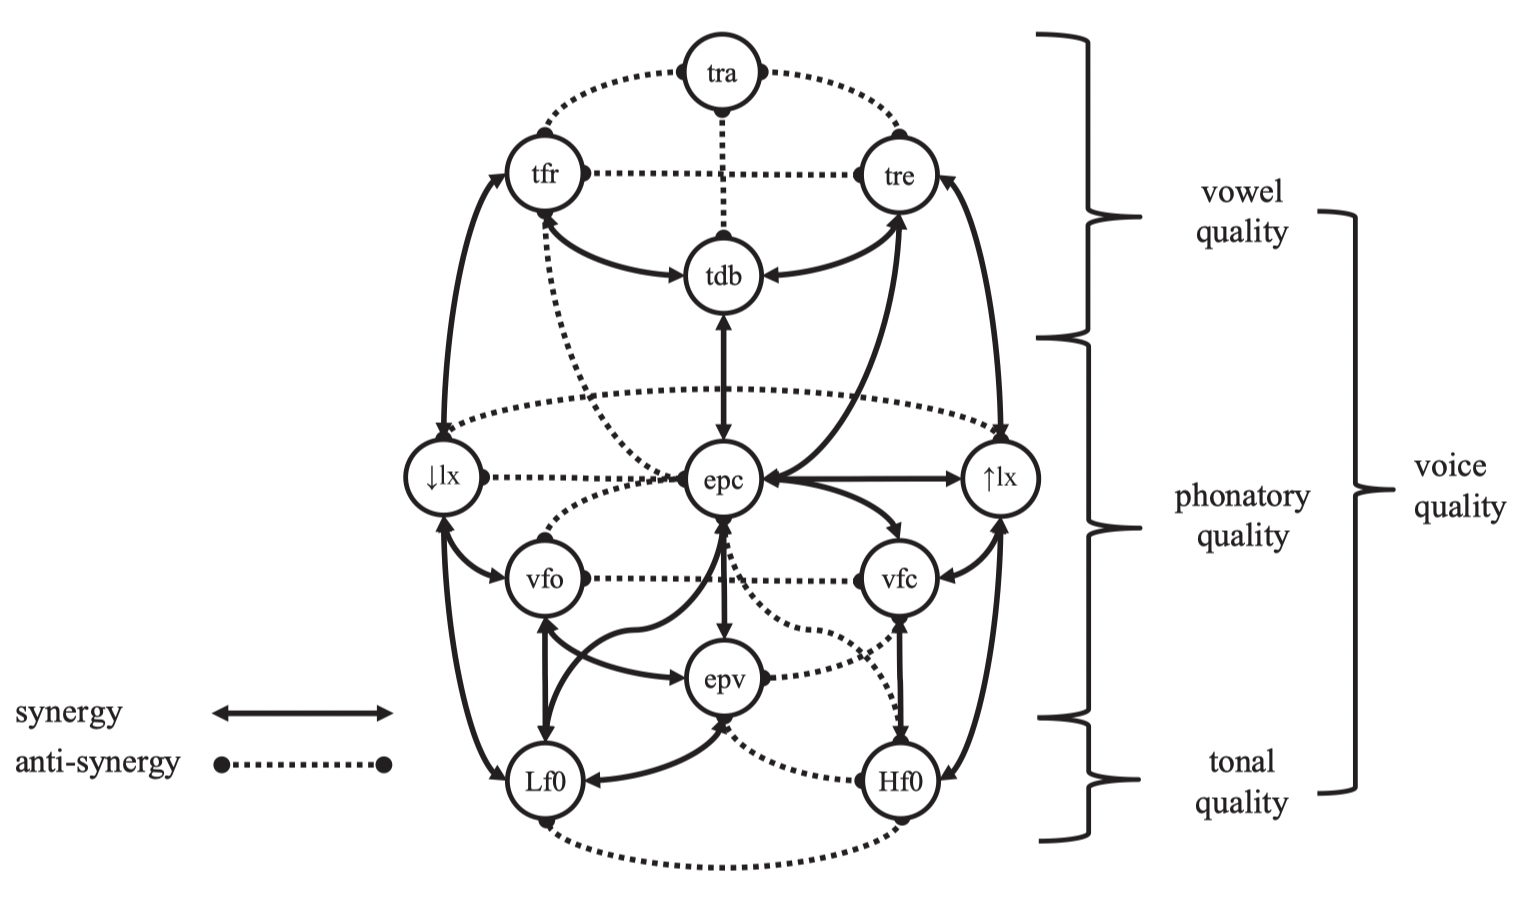
\includegraphics[width=0.9\textwidth]{../LAMNetwork.png}
	\caption{Network of synergistic and anti-synergistic nodes in the Laryngeal Articulator Model. Taken from \citet{eslingVoiceQualityLaryngeal2019}.}
	\label{fig:LAMNetwork}
\end{figure}
	
Figure~\ref{fig:LAMNetwork}, shows which nodes interact in synergistic and anti-synergistic ways. This network is divided into three parts that represent the nodes which are responsible for vowel quality, phonatory quality, and tonal quality. For example, the node `epc' which is one of the nodes responsible for phonatory quality (i.e., responsible for producing phonation) has synergistic relationships with the nodes representing larynx raising (↑lx), vocal fold closure (vfc), tongue bunching(tdb), tongue retraction (tre), and for decreasing the vocal fold mass leading to a lowering of f0 (Lf0). In contrast this same node has anti-synergistic relationships with tongue fronting (tfr), larynx lowering (↓lx), vocal fold opening (vfo), and increasing vocal fold tension which leads to less vibrating mass and an increase to f0 (Hf0). This means that when there is epilaryngeal constriction there is an increased chance for the synergistic relationships to also co-occur. However, this does not mean that the synergistic nodes must co-occur when the node is activated. 

While \posscitet{eslingVoiceQualityLaryngeal2019} Laryngeal Articulator Model does make a compelling argument for the complexity of the larynx and allows for a detailed account of what the larynx is doing during phonation, it is not entirely clear if this added complexity is altogether warranted. From the results of the statistical analysis the simplified one-dimensional model of the larynx is fully capable of explaining the behavior we observe in SLZ and the other Oto-Manguean languages which form the backbone of the LCH. If, however, we were observe large degrees of overlap between tone and phonation then it stands to reason that the LCH does not capture the nature of the laryngeal systems we are observing and a different model of the larynx, such as the Laryngeal Articulator Model, is needed to capture the more complex interactions of tone and phonation. 

%------------------------------------
\section{Conclusion} \label{sec:Conclusion}
%------------------------------------

In conclusion, this paper has provided a brief introduction to the tonal and phonation systems of Santiago Laxopa Zapotec, an understudied variety of Sierra Norte Zapotec. This system is important for studying the interaction of tone and phonation because of the complex interactions between tone and phonation that are found in this language. Because any phonation type can co-occur with any tone this presented a unique opportunity to see how the language compensates for using larynx for both tone and phonation. This paper has shown by using language data that was collected from elicitation data that the Laryngeal Complexity Hypothesis presented by \citet{silvermanLaryngealComplexityOtomanguean1997} and \citet{blankenshipTimeCourseBreathiness1997, blankenshipTimingNonmodalPhonation2002} appears to be the best model of accounting for how tone and phonation interact. 

The Laryngeal Complexity Hypothesis states that when a language has both tone and phonation these two components of the vowel are ordered or phased with respect to one another. The reason that this phasing occurs is to allow for the greatest amount of perceptibility in the acoustic signal. This allows the listener to adequately interpret the acoustic signals for tone and phonation. 

This ability of speakers to interpret the acoustic signals in conjunction with the acoustic signals for tone is of great interest and would benefit from a perception experiment to determine what it is that the speakers are using to differentiate the different phonation types. This is especially true for laryngealized vowels which have such a varied pronunciation. 

This study will benefit from further analysis and data collection. Now that the world is in a safer state in regards to COVID-19 it is important to collect data from more speakers to corroborate the data and analysis from FSR and RD. 



%------------------------------------
%BIBLIOGRAPHY
%------------------------------------

%\singlespacing
% \nocite{*}
\printbibliography[heading=bibintoc]

\end{document} 